\documentclass{article}

\usepackage[square,sort,comma,numbers]{natbib}
\usepackage{amsmath}
\usepackage{graphicx}
\usepackage{../sty/arxiv}
\usepackage{setspace}
\usepackage[utf8]{inputenc} % allow utf-8 input
\usepackage[T1]{fontenc}    % use 8-bit T1 fonts
\usepackage{hyperref}       % hyperlinks
\usepackage{url}            % simple URL typesetting
\usepackage{booktabs}       % professional-quality tables
\usepackage{amsfonts}       % blackboard math symbols
\usepackage{nicefrac}       % compact symbols for 1/2, etc.
\usepackage{microtype}      % microtypography
\usepackage{lipsum}
\usepackage{mathtools}
\usepackage{epigraph}
\usepackage{csquotes}

\usepackage{listings}       % added for codeblock
\usepackage{xcolor}         % added for syntax highlighting

\newcommand{\norm}[1]{\left\lVert#1\right\rVert}

\begin{document}

% front matter
\title{Beyond Zero-Shot: A Hierarchical Approach To Multi-Agent Collaboration For Improved LLM Accuracy}

\author{
    \bf Giovanpaolo Vrenna \\ \texttt{Giovanpaolo.vrenna@keio.jp} \\
    \and
    \bf Shigeki Noguchi \\ \texttt{noguchi\_shigeki@keio.jp} \\
    \and
    \bf Naoki Watson \\ \texttt{naokiwatson@keio.jp} \\
    \and
    \bf Keita Fujie \\ \texttt{fk77663@keio.jp} \\
}

\date{}
\maketitle
\onehalfspacing

\begin{abstract}
    When Large Language Model agents engage in debate, they collectively enhance their intelligence. This study explores the impact of hierarchical communication structures on multi-agent debate systems, introducing two distinct hierarchical topologies along with a method for their implementation. Our results indicate that these structures improve reasoning performance, achieving approximately 20\% higher accuracy compared to zero-shot agents. Additionally, we conducted a comparative analysis of shallow and deep hierarchical topologies. While our findings do not explicitly reveal a performance difference, our analysis of conversation history suggests that deeper hierarchical structures introduce greater redundancy in the reasoning process, which may, in turn, enhance self-correction
\end{abstract}


% sections
\section{Introduction}
\label{sec:introduction}

Since the introduction of the transformer architecture in 2017\cite{vaswani2023attentionneed} and the release of OpenAI’s GPT models\cite{radford2018improving}\cite{radford2019language}\cite{brown2020languagemodelsfewshotlearners}, the machine learning community has primarily focused on transformer-based models. The discovery of scaling laws\cite{kaplan2020scalinglawsneurallanguage} further shifted research priorities from optimizing model efficiency to increasing model and dataset sizes. As models were trained on vast datasets sourced from the internet, scaling laws initially continued to hold, but their limitations have since been questioned. While it remains uncertain whether these laws have truly reached a ceiling, it is evident that most publicly available raw text data has already been utilized. Consequently, research efforts begun shifting toward improving model inference quality. As of February 2025, DeepSeek R1, one of the leading models known for its strong reasoning capabilities, had been further refined through reinforcement learning\cite{deepseekai2025deepseekr1incentivizingreasoningcapability}. Post-training techniques for foundational models have become vital for achieving high reasoning performance.

Moreover, recent research demonstrates that LLMs can achieve enhanced performance through techniques like prompt engineering, without updating model weights. For example, Chain of Thought (CoT) reasoning\cite{kojima2023largelanguagemodelszeroshot} improves an LLM’s ability to solve complex problems by simply instructing it to “think step by step.” Similarly, reflection prompting\cite{madaan2023selfrefineiterativerefinementselffeedback}\cite{shinn2023reflexionlanguageagentsverbal} models to think about their own thinking before finalizing an answer—has proven effective in refining their reasoning capabilities. Moreover, employing a multi-agent debate strategy, where several LLM agents engage in structured discussions, has been shown to further boost performance compared to a single-agent approach \cite{du2023improvingfactualityreasoninglanguage}.

In this study, we analyzed the performance of different multi-agent debate system hierarchies. Specifically, we compared the effectiveness of a zero-shot agent against various multi-agent configurations, assessing their impact on accuracy, computational cost, and time efficiency. Our findings provide insights into the trade-offs associated with different debate structures and highlight the advantages of multi-agent collaboration in enhancing reasoning capabilities. Furthermore, we discuss adaptive hierarchical structures that dynamically evolve based on performance metrics for more accurate multi-agent reasoning frameworks.

\section{Background}
\label{sec:background}

Collective intelligence refers to the phenomenon where the combined capabilities of multiple individuals or agents—whether human or machine—yield problem-solving and decision-making outcomes that surpass those of any single participant. In the context of large language models, Du et al(2023)\cite{du2023improvingfactualityreasoninglanguage} explored their collective performance within a multi-agent debate system. The debate workflow follows these steps:
\begin{enumerate}
\item Given a question, multiple agents generate independent answers.
\item Agents review each other’s responses and reasoning.
\item Each agent revises its response based on feedback from others.
\item This iterative process continues for multiple rounds.
\end{enumerate}

The communication topology in the study was fully connected, meaning each agent had access to all other agents’ responses at every debate round. There was no hierarchical structure, and all agents played an equal role in refining their answers. Instead of fixed pairwise debates, responses were broadcast to all agents, allowing them to critique and update their reasoning iteratively. This setup facilitated iterative consensus formation, where incorrect or uncertain answers were gradually refined. The debate process did not rely on a central judge or leader; instead, all agents contributed equally.

The study evaluated the multi-agent debate framework across six benchmarks covering reasoning and factual accuracy tasks. For reasoning, they tested arithmetic expressions, grade school math (GSM8K), and chess move prediction, measuring accuracy and logical consistency. For factual accuracy, they assessed biography generation, MMLU (Massive Multitask Language Understanding), and chess move validity, testing the correctness of generated facts. The multi-agent debate consistently outperformed single-agent approaches, self-reflection methods, and majority voting as summarized in Figure~\ref{fig:multiagent}.
\begin{figure}
    \centering
    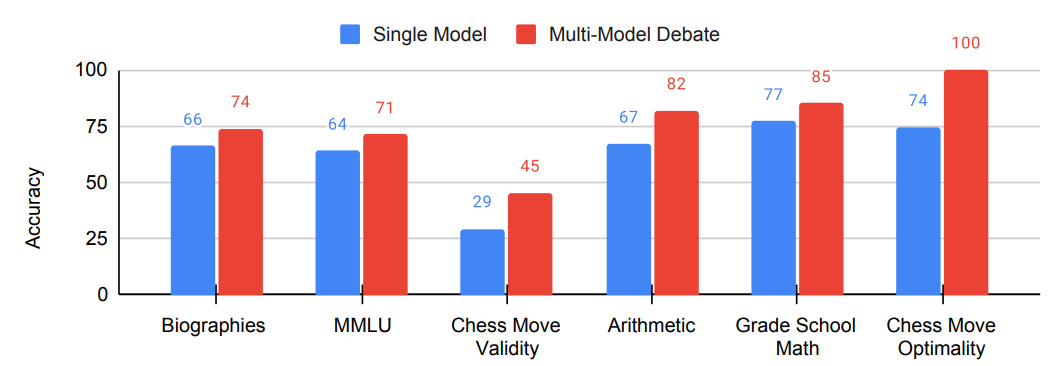
\includegraphics[width=1\linewidth]{img/section_background/multi-agent-debate-result.png}
    \caption{{Multiagent Debate Improves Reasoning and Factual Accuracy}}
    \label{fig:multiagent}
\end{figure}

Although this result is surprising, the performance of the multi-agent debate system plateaus as the number of agents or rounds increases, eventually converging to a certain level (see Figure \ref{fig:performance_with_increased}). Based on these observations, we hypothesize that incorporating dynamic, hierarchical communication topologies could further enhance the system. To implement the debate system and its communication topology, we leveraged the Autogen framework\cite{microsoft_autogen}, which provides the flexibility to define both the topology and the agents’ behavior.
\begin{figure}
    \centering
    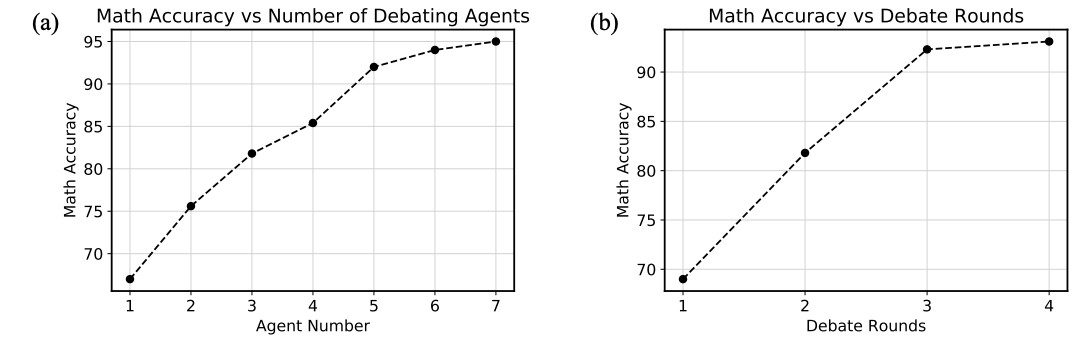
\includegraphics[width=0.85\linewidth]{img/section_background/performance_with_increased.png}
    \caption{(a) Performance with Increased Agents. (b) Performance with Increased Rounds}
    \label{fig:performance_with_increased}
\end{figure}
\section{Implementation}
\label{sec:implementation}

\subsection{Framework: Microsoft AutoGen}
AutoGen is a multi-agent framework developed by Microsoft. It offers natively a more flexible agent topology, enhanced LLM inference, and dynamic agent collaboration. These features enable us to build a more robust and flexible multi-agent system \cite{microsoft_autogen}.

These are the key components of AutoGen that we used in our project:
\begin{itemize}
    \item \textbf{ConversableAgent:} In AutoGen's framework, the ConversableAgent class serves as a customizable foundation for agents capable of engaging in conversations with other agents, humans, and tools to accomplish tasks collaboratively.
    \item \textbf{GroupChat:} A GroupChat is a collection of agents that can communicate with each other.
    \item \textbf{GroupChatManager:} In AutoGen's multi-agent group chat, the GroupChatManager plays a major role in facilitating agent communication. When an agent generates a response, the GroupChatManager broadcasts it to all participating agents in GroupChat. This broadcasting mechanism ensures that all agents remain informed of the ongoing conversation, allowing them to contribute effectively to collaborative tasks. The GroupChatManager also manages the flow of the conversation by selecting the next speaker, by orchestrating a coherent and organized dialogue among the agents.
    \item \textbf{SocietyOfMindAgent:} The Society of Mind Agent in Microsoft's AutoGen framework is inspired by Marvin Minsky's “Society of Mind” theory, which posits that intelligence emerges from the interactions of simple, mindless agents working together. In AutoGen, the Society of Mind Agent can orchestrate and wrap GroupChat and GroupChatManager objects that host agents and debates. Externally, it functions as a singular cohesive agent and the conversation within GroupChat under the SocietyOfMindAgent can be considered an "Inner Dialogue". This internal discourse allows for the weighing of options and the integration of multiple viewpoints, ultimately guiding behavior and thought processes.
\end{itemize}

\subsection{Code}
The code introduced a dynamic hierarchy system where a hierarchy string (e.g., “ABB”) defines the structure of a group of agents. Each letter in the hierarchy string represents the nodes that consists of agents such as the Prompt Generator, Counter, Working Agent, Checker, and Subordinate Nodes. The hierarchy system allows a clear definition of the agent hierarchy, a flexible representation of the topology, and an optimized information flow. 

\subsubsection{Agents}
\textbf{Prompt Generator:} The Prompt Generator is responsible for structuring and reformatting the problem before any agent attempts to solve it. It does not solve the problem itself but ensures that agents receive a clear and well-defined prompt.

\textbf{Counter:} The Counter Agent is responsible for tracking the number of debate rounds and ensuring the conversation does not continue indefinitely. It does not contribute to the discussion but simply counts rounds and signals progress.

\textbf{Working Agent:} The Working Agents are responsible for solving the problem based on the structured prompt. They generate initial solutions, review responses from other agents, and refine their answers through debate.

\textbf{Checker:} The Checker Agent is responsible for evaluating whether the Subordinate Agents' answers are converged. It does not solve the problem—instead, it decides whether the answers agree or if further rounds are needed. It can terminate or continue the debate based on the convergence of responses.

\textbf{Subordinate Nodes:} The Subordinate Nodes are nested within the SocietyOfMindAgent(s). These consist of the Prompt Generator, Counter, Working Agents, Checker, and Subordinate Nodes if these nodes host further subnodes. 

\subsubsection{Hierarchy String Conversion Rules}
The hierarchy string needs to be processed by a function to convert it into a multi-agent topology. The function is \textit{parse\_subnodes\_generic(letters)} that takes a string of letters as input and returns a list of subnodes. The function follows these rules:

\textbf{Rule 1: Identifying Generations (Levels of Hierarchy)}

The hierarchy is built by identifying distinct levels (generations) of agents, based on letter occurrences. The earliest occurring letter (lexicographically lowest) (e.g., 'A') is designated as Generation 0. Subsequent letters define child nodes of the previous generation, forming hierarchical relationships. Each new letter appearing after a previous letter indicates a transition to a lower level (subordinate node). 

For instance, the string is "ABC": $$"ABC" \rightarrow Gen\_0:A \rightarrow Gen\_1:B \text{(Subordinate to A)} \rightarrow Gen\_2:C \text{(Subordinate to B)}$$

\textbf{Rule 2: Grouping Subordinate Nodes}

For each identified generation, consecutive occurrences of the same letter are grouped under a common parent node. These grouped nodes operate within the same hierarchical layer and are peers within the structure.

\textbf{Rule 3: Parent-Child Relationships}

A letter that appears after another letter of the same or a lower level is assigned as its child. A new letter that appears after the lowest-ranked letter (earliest in order) indicates the start of a new group.

\textbf{Rule 4: Tracking Generations Dynamically}

The function dynamically tracks each letter’s depth in the hierarchy, ensuring that sibling nodes are grouped correctly, child nodes are assigned to the appropriate parent, and the overall hierarchical structure is accurately maintained.

\textbf{Rule 5: Handling Nested Hierarchies (Recursive Parsing)}

If a letter appears at a deeper level than its immediate predecessor, it belongs to a subordinate node. The function recursively parses the hierarchy to establish nested societies of mind.

\textbf{Rule 6: Assigning Subnode Identifiers}

Subordinate nodes are labeled with unique identifiers based on their structure. If a node is part of a repeated pattern, a numerical suffix is assigned to distinguish between different instances. If the string is "ABCCBCC", the subnode identifiers would be "ABB1" representing the first instance of BB under A, and "BCC1", and "BCC2" indicating two separate groups of BCC under different parent nodes.

\textbf{Example:}

Given the hierarchy string "ABCCBCCCABCDDCBCCDEEDEEC" and "ABCDEEDCDDDBCCBCDDCCB", the function would parse the hierarchy like these network diagrams in Figure ~\ref{fig:ABCCBCCCABCDDCBCCDEEDEEC} and Figure ~\ref{fig:ABCDEEDCDDDBCCBCDDCCB}

\begin{figure}[h]
    \centering
    \begin{minipage}{0.49\linewidth}
        \centering
        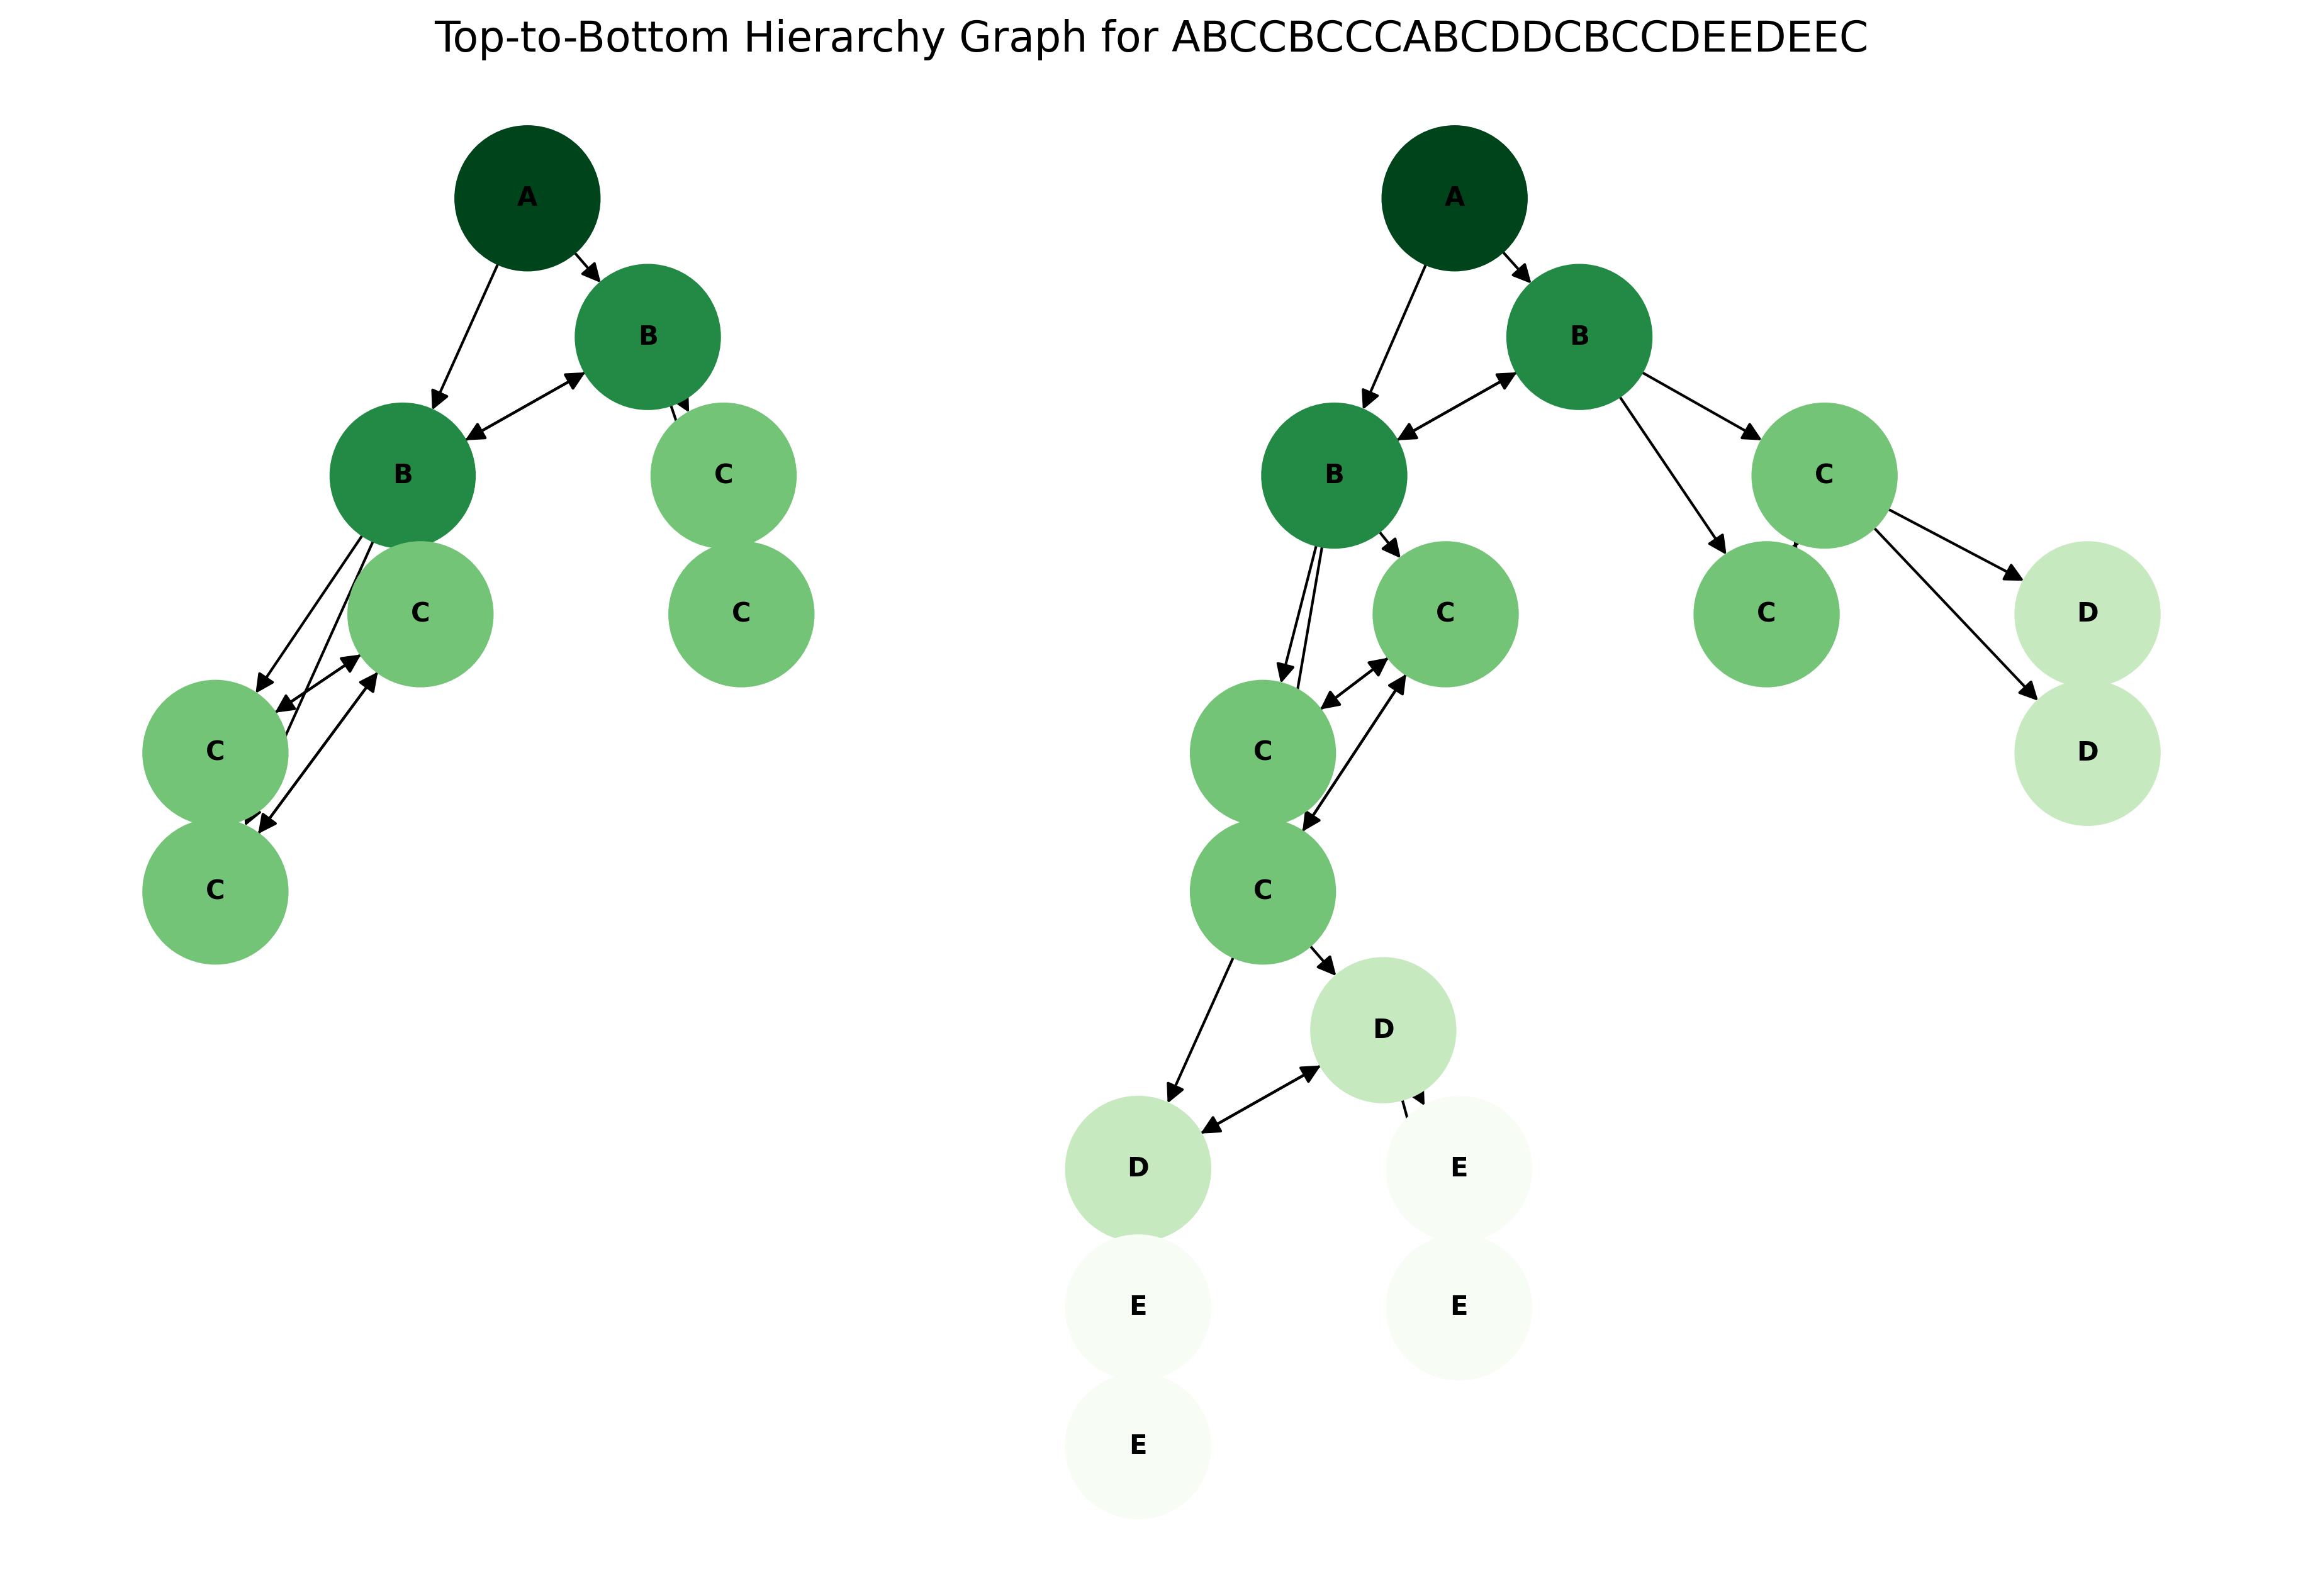
\includegraphics[width=\linewidth]{img/section_implement/ABCCBCCCABCDDCBCCDEEDEEC.png}
        \caption{Visualization of the hierarchy string "ABCCBCCCABCDDCBCCDEEDEEC"}
        \label{fig:ABCCBCCCABCDDCBCCDEEDEEC}
    \end{minipage}
    \hfill
    \begin{minipage}{0.49\linewidth}
        \centering
        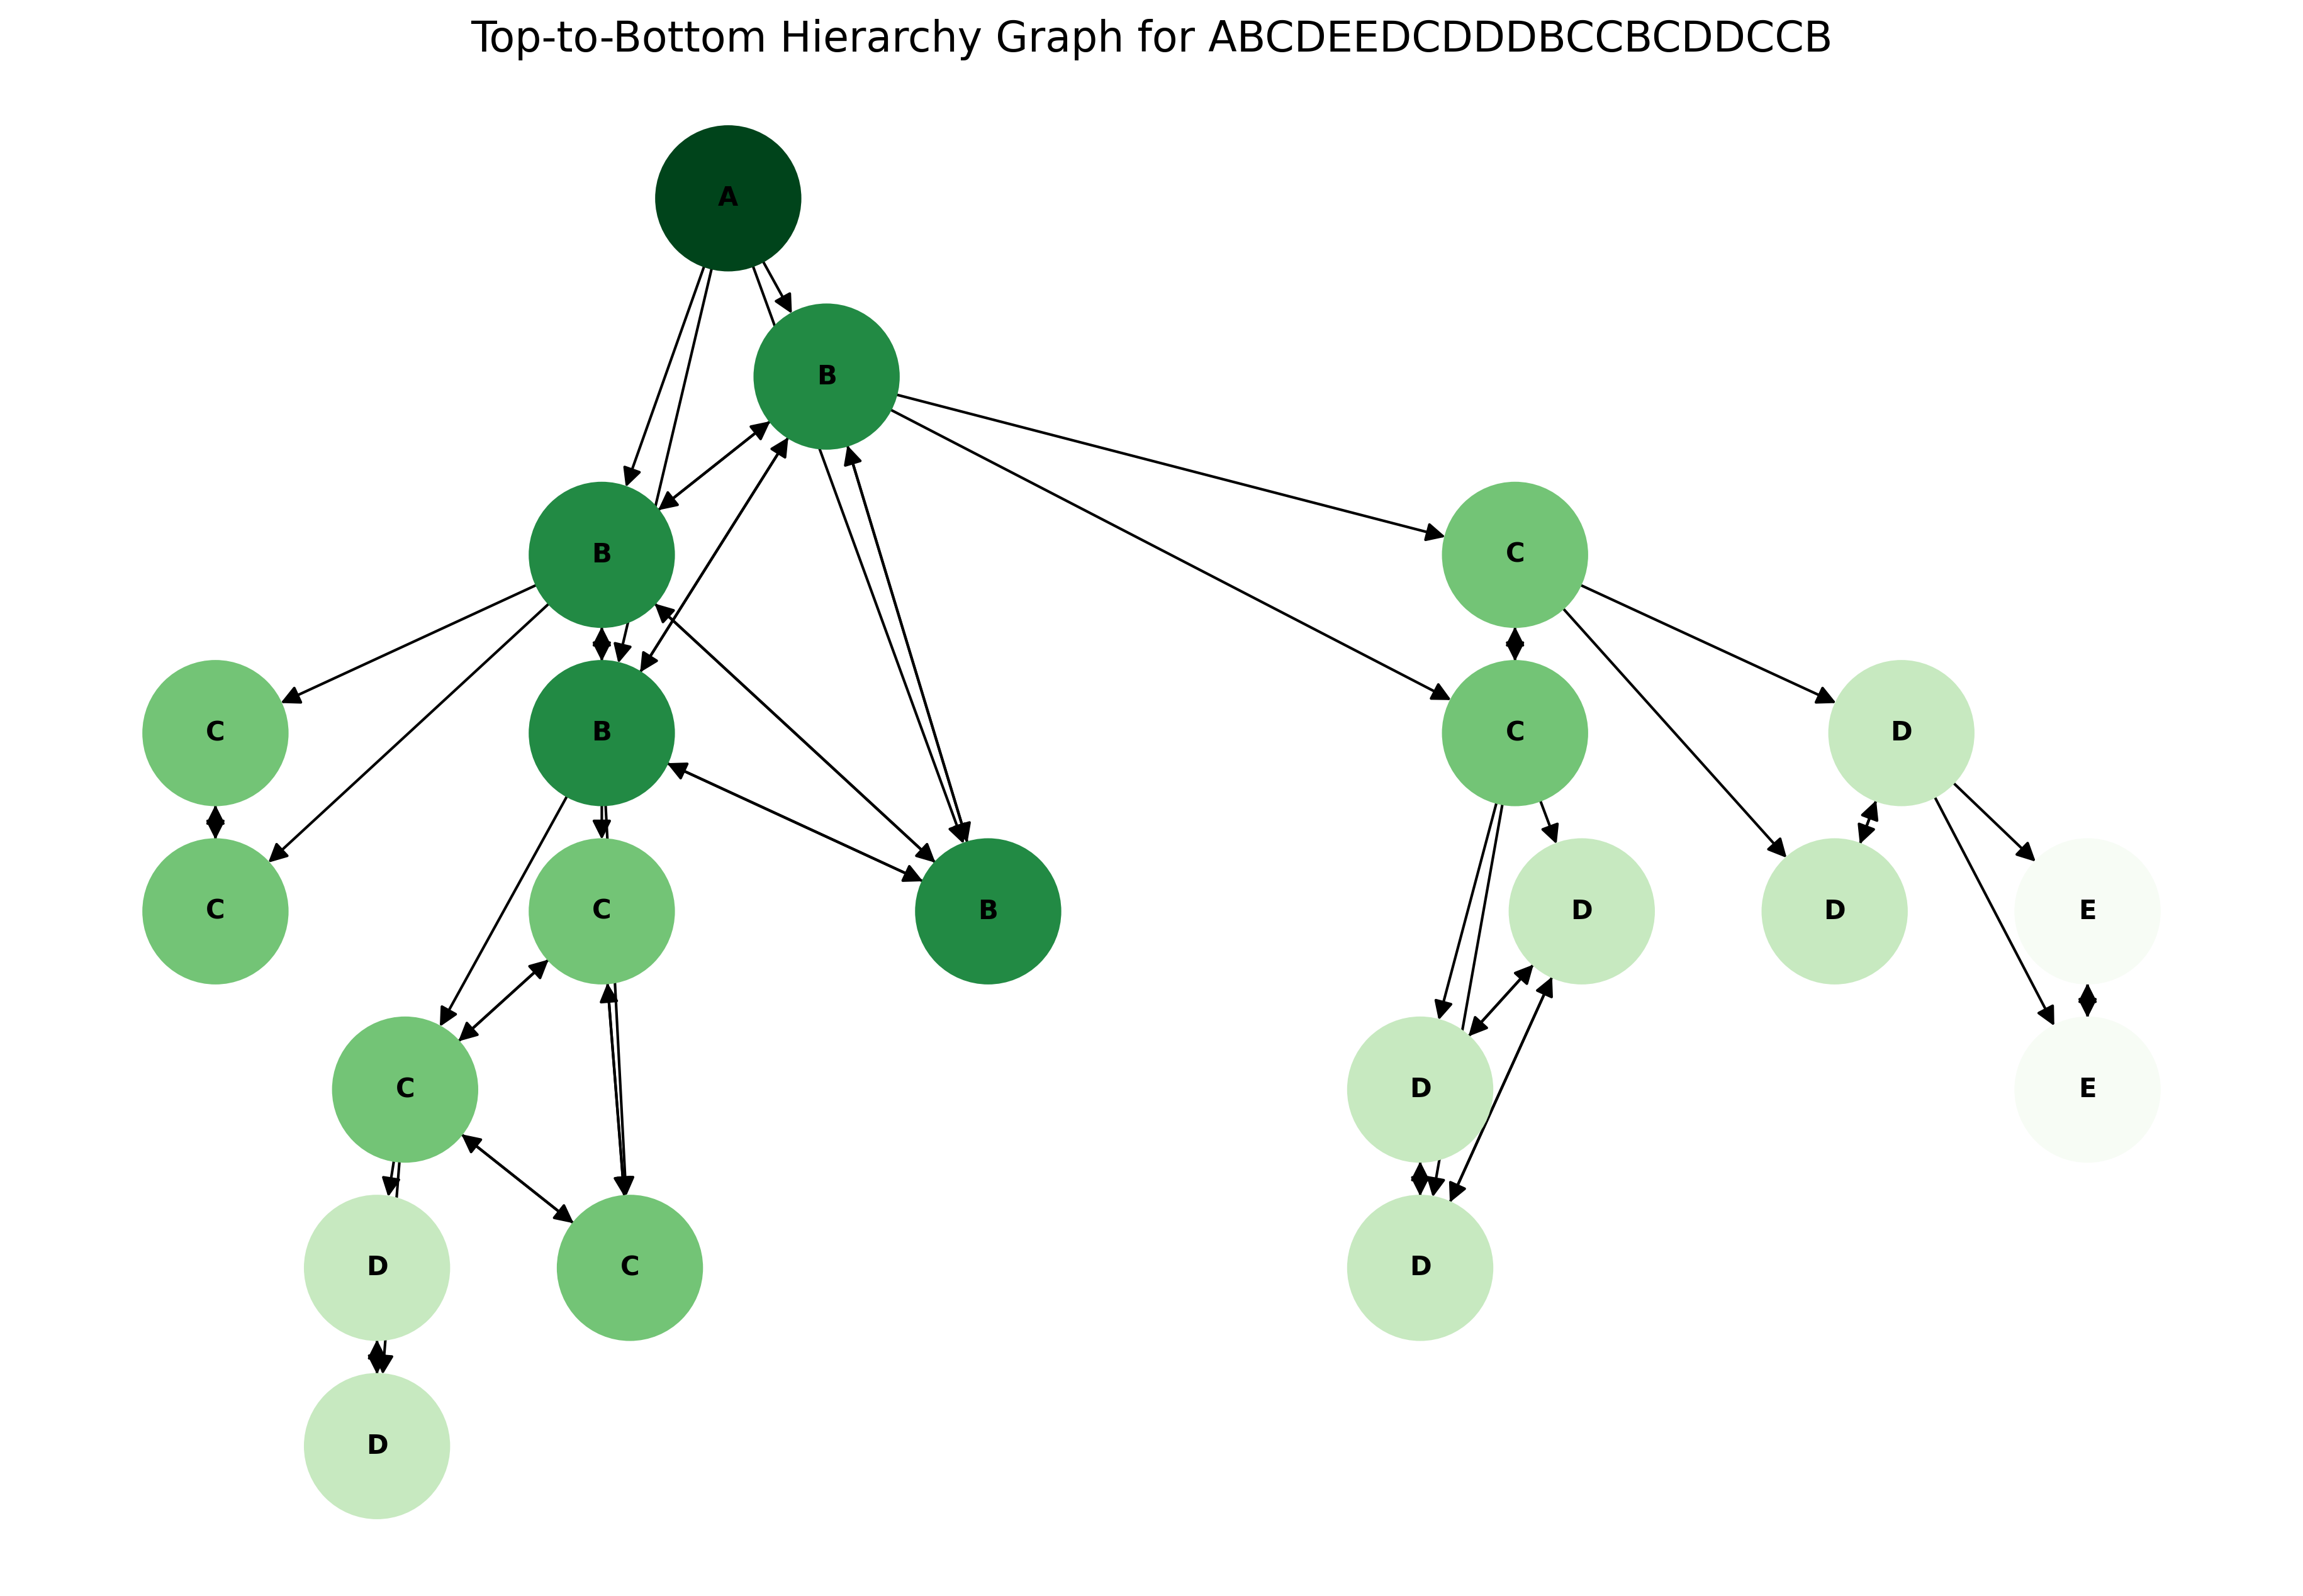
\includegraphics[width=\linewidth]{img/section_implement/ABCDEEDCDDDBCCBCDDCCB.png}
        \caption{Visualization of the hierarchy string "ABCDEEDCDDDBCCBCDDCCB"}
        \label{fig:ABCDEEDCDDDBCCBCDDCCB}
    \end{minipage}
\end{figure}

\subsubsection{Workflow}

The system operates by:
\begin{enumerate}
\item \textbf{Parsing the Hierarchy String:} The hierarchy string is processed to identify generations (Gen\_0, Gen\_1, ..., Gen\_i ..., Gen\_n), where each generation corresponds to a distinct group of agents.
\item \textbf{Forming Subnodes:} Each subnode is treated as an independent GroupChat, hosting its own set of agents (Prompt Generator, Counter, Working Agents, and Checker). These agents engage in structured discussions within their designated subnode. The nodes/subnodes are created dynamically based on the hierarchy string.
\item \textbf{Nested Debate and Refinement:} The debate starts at the lowest level (Gen\_0), where Working Agents produce initial solutions. As discussions progress, higher-generation (Gen\_i) subordinate subnodes generate the responses, leading to a hierarchical refinement of answers.
\item \textbf{Top-Down Control \& Bottom-Up Aggregation:} The Supreme Hierarchy SocietyOfMindAgent oversees the entire hierarchy, ensuring that responses from lower generations are aggregated and passed upwards, while high-level decisions cascade down to guide subnode debates.
\end{enumerate}

This hierarchical grouping approach optimizes communication, prevents redundant discussions across unrelated agents, and ensures that information flows efficiently between different levels of the system. The combination of structured debates, iterative refinement, and dynamic agent organization enables the framework to produce well-reasoned, high-quality, accurate responses.
\section{Experiment Setup and Testing Methodology}
\label{sec:methodology}

The objective of this experiment is to evaluate the performance of these multi-agent AI systems and observe its accuracy in solving a multitude of mathematical problems. These results will be compared to the performance of a single AI agent in order to contextualize these results and show the difference in accuracy, efficiency, and scalability of these different approaches.

This hierarchical debate system is important because LLMs are known to occasionally produce incorrect and inconsistent responses. The goal of this experimentation is to show whether the hierarchical debate system and iterative refinement would lead to more accurate and reliable outputs. More specifically, this experiment aims to evaluate whether hierarchy depth further increases the accuracy at which the sample questions are answered.

\subsection{Test 1: Smaller Hierarchy}
The first test is designed to test a zero-shot AI agent against a multi-agent hierarchical system, following the "ABB" structure. This structure consists of one primary subnode, with two subordinate agents in the subnode. There are also support agents, those being the Prompt Generator, Counter, Checker, and Chat Manager.

\begin{figure}[h]
    \centering
    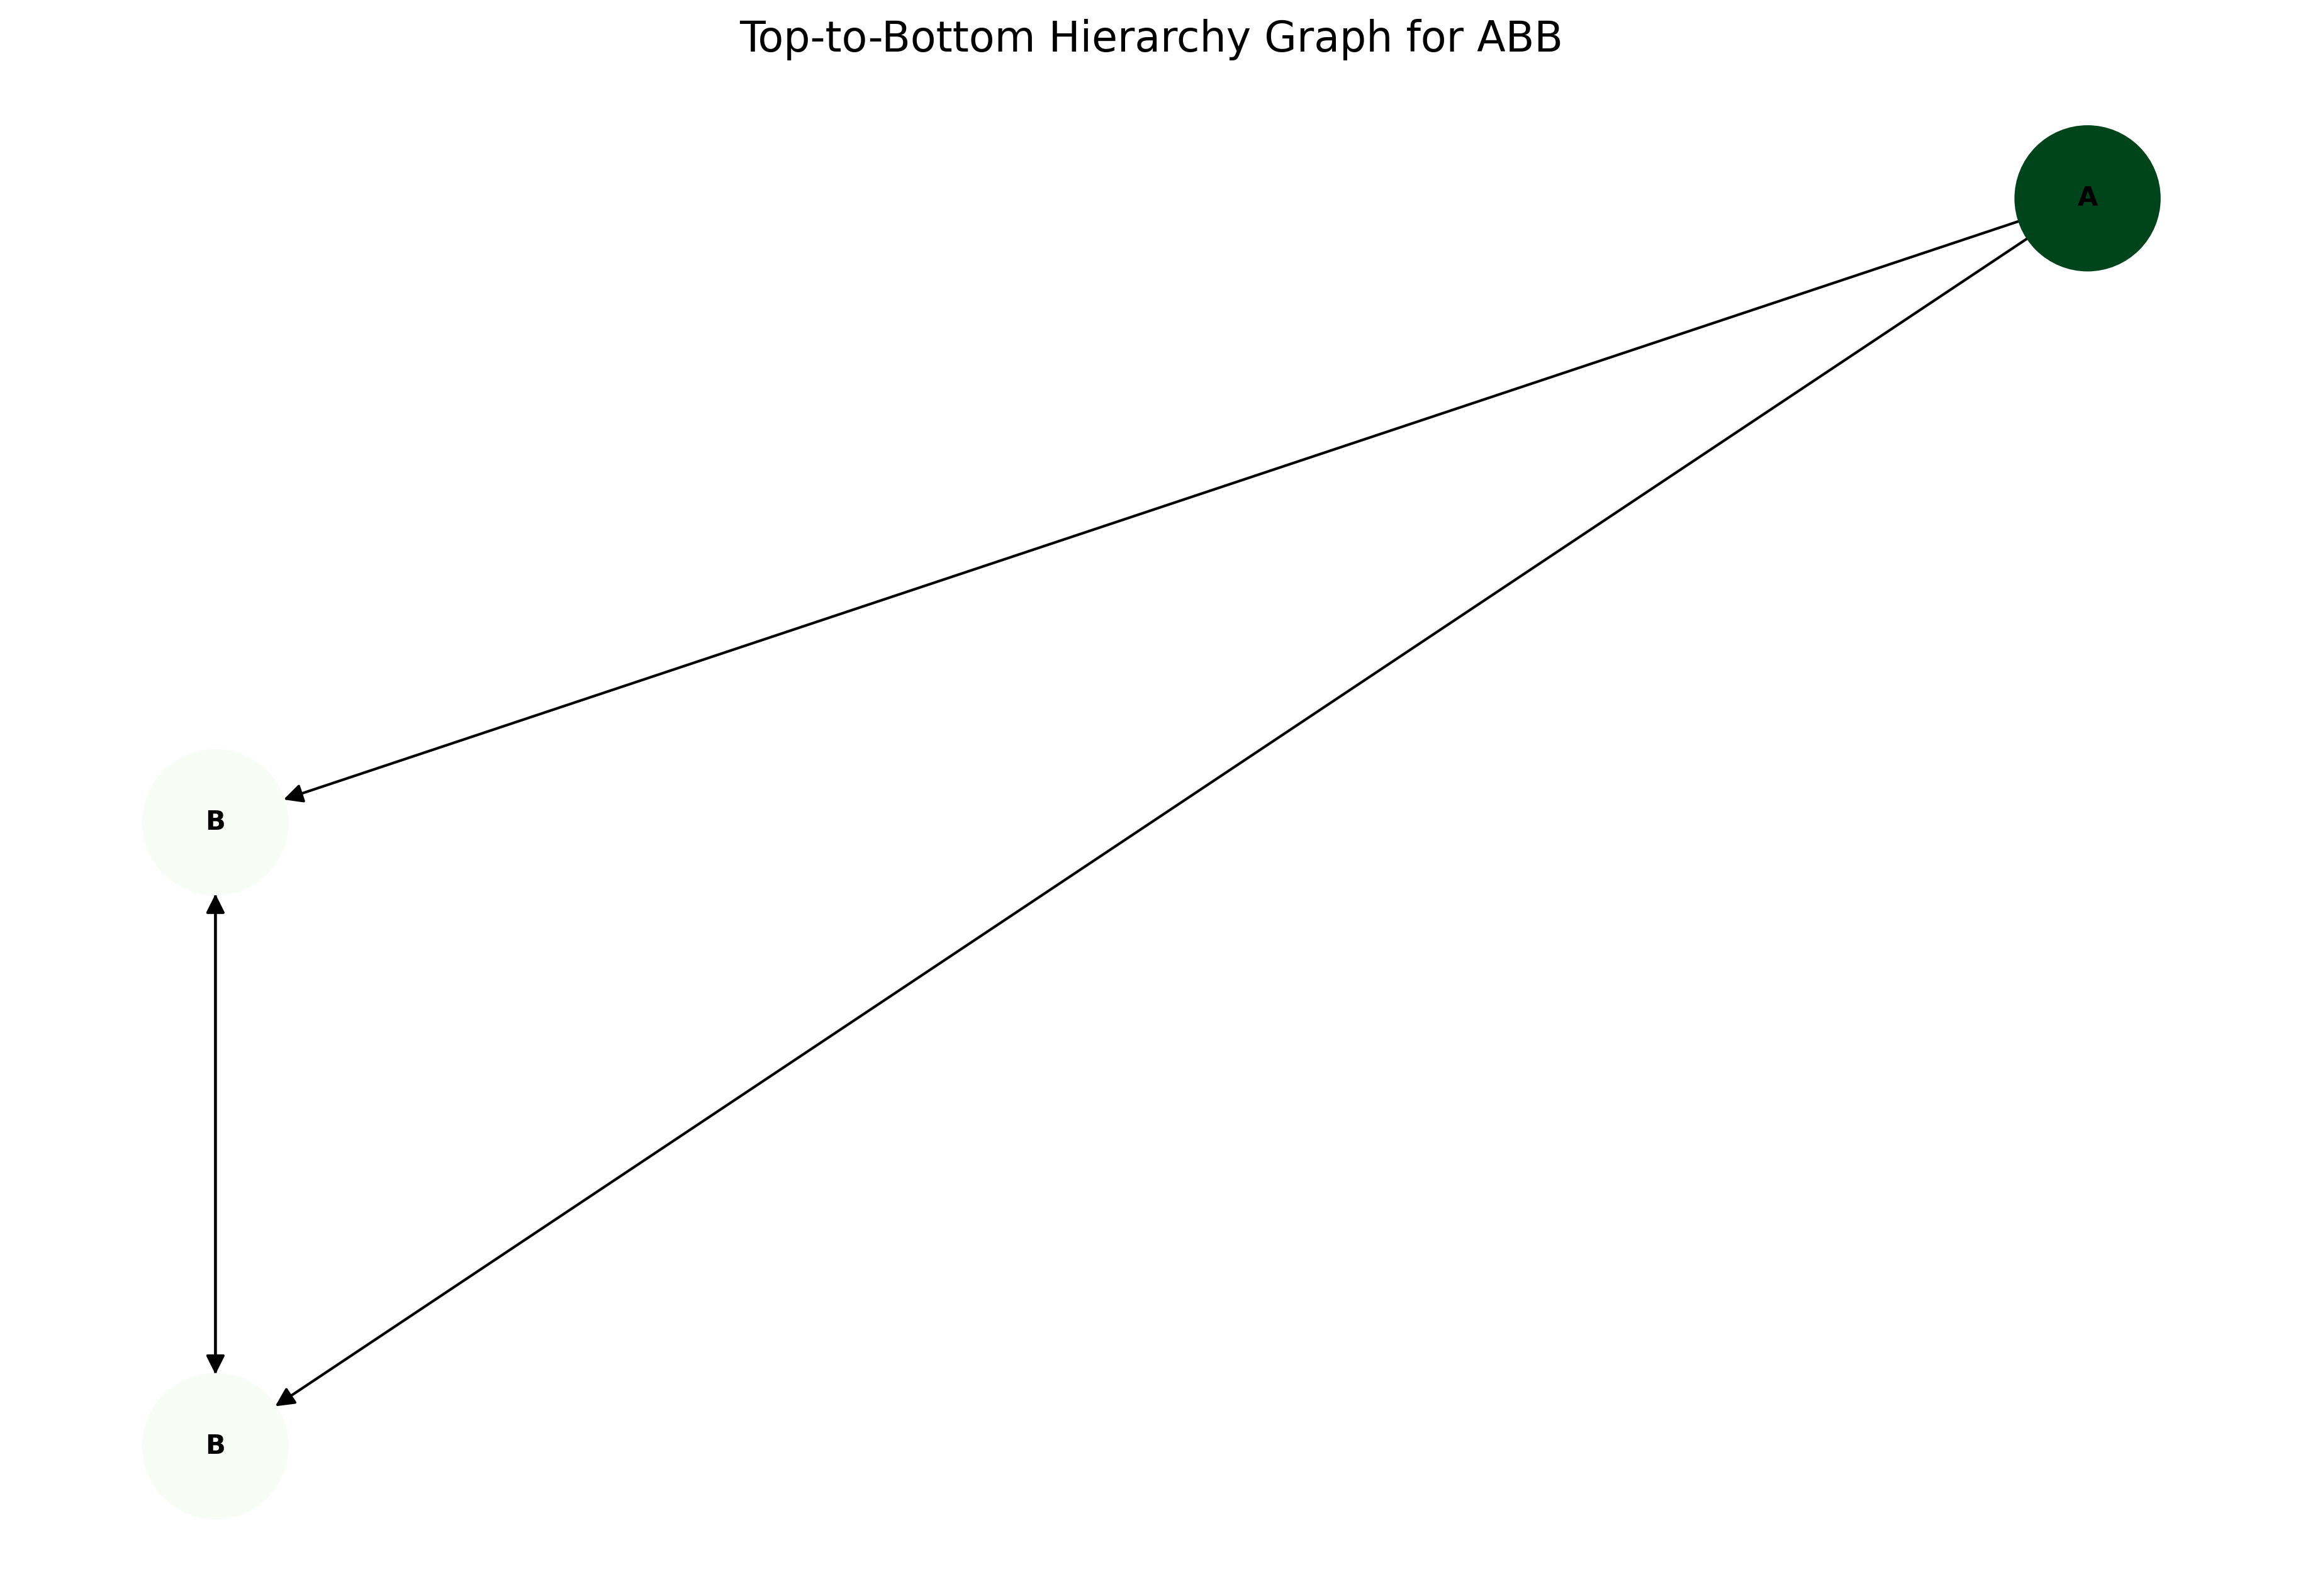
\includegraphics[width=0.8\textwidth]{img/section_methodology/ABB.png}
    \caption{A Visualization of the Smaller "ABB" Hierarchy}
    \label{fig:smaller}
\end{figure}

Both the zero-shot AI agent and the "ABB" multi-agent hierarchy will be tasked with solving a set of 1000 questions, and then checked against an answer key. This experiment will establish a baseline comparison between the zero-shot agent and the simple-hierarchy multi-agent system. This will establish the effect of a small amount of collaboration between agents on solving problems. 

\subsection{Test 2: Large Hierarchy}
Similarly to the first test, this second test will evaluate the performance of a zero-shot AI agent compared to a hierarchical system. However, this will be with the more complex hierarchical structure "ABCCBCCC". This structure has one Gen 0 subnode, two Gen 1 subnodes, seven subordinate agents, and then the same support agents. 

\begin{figure}[h]
    \centering
    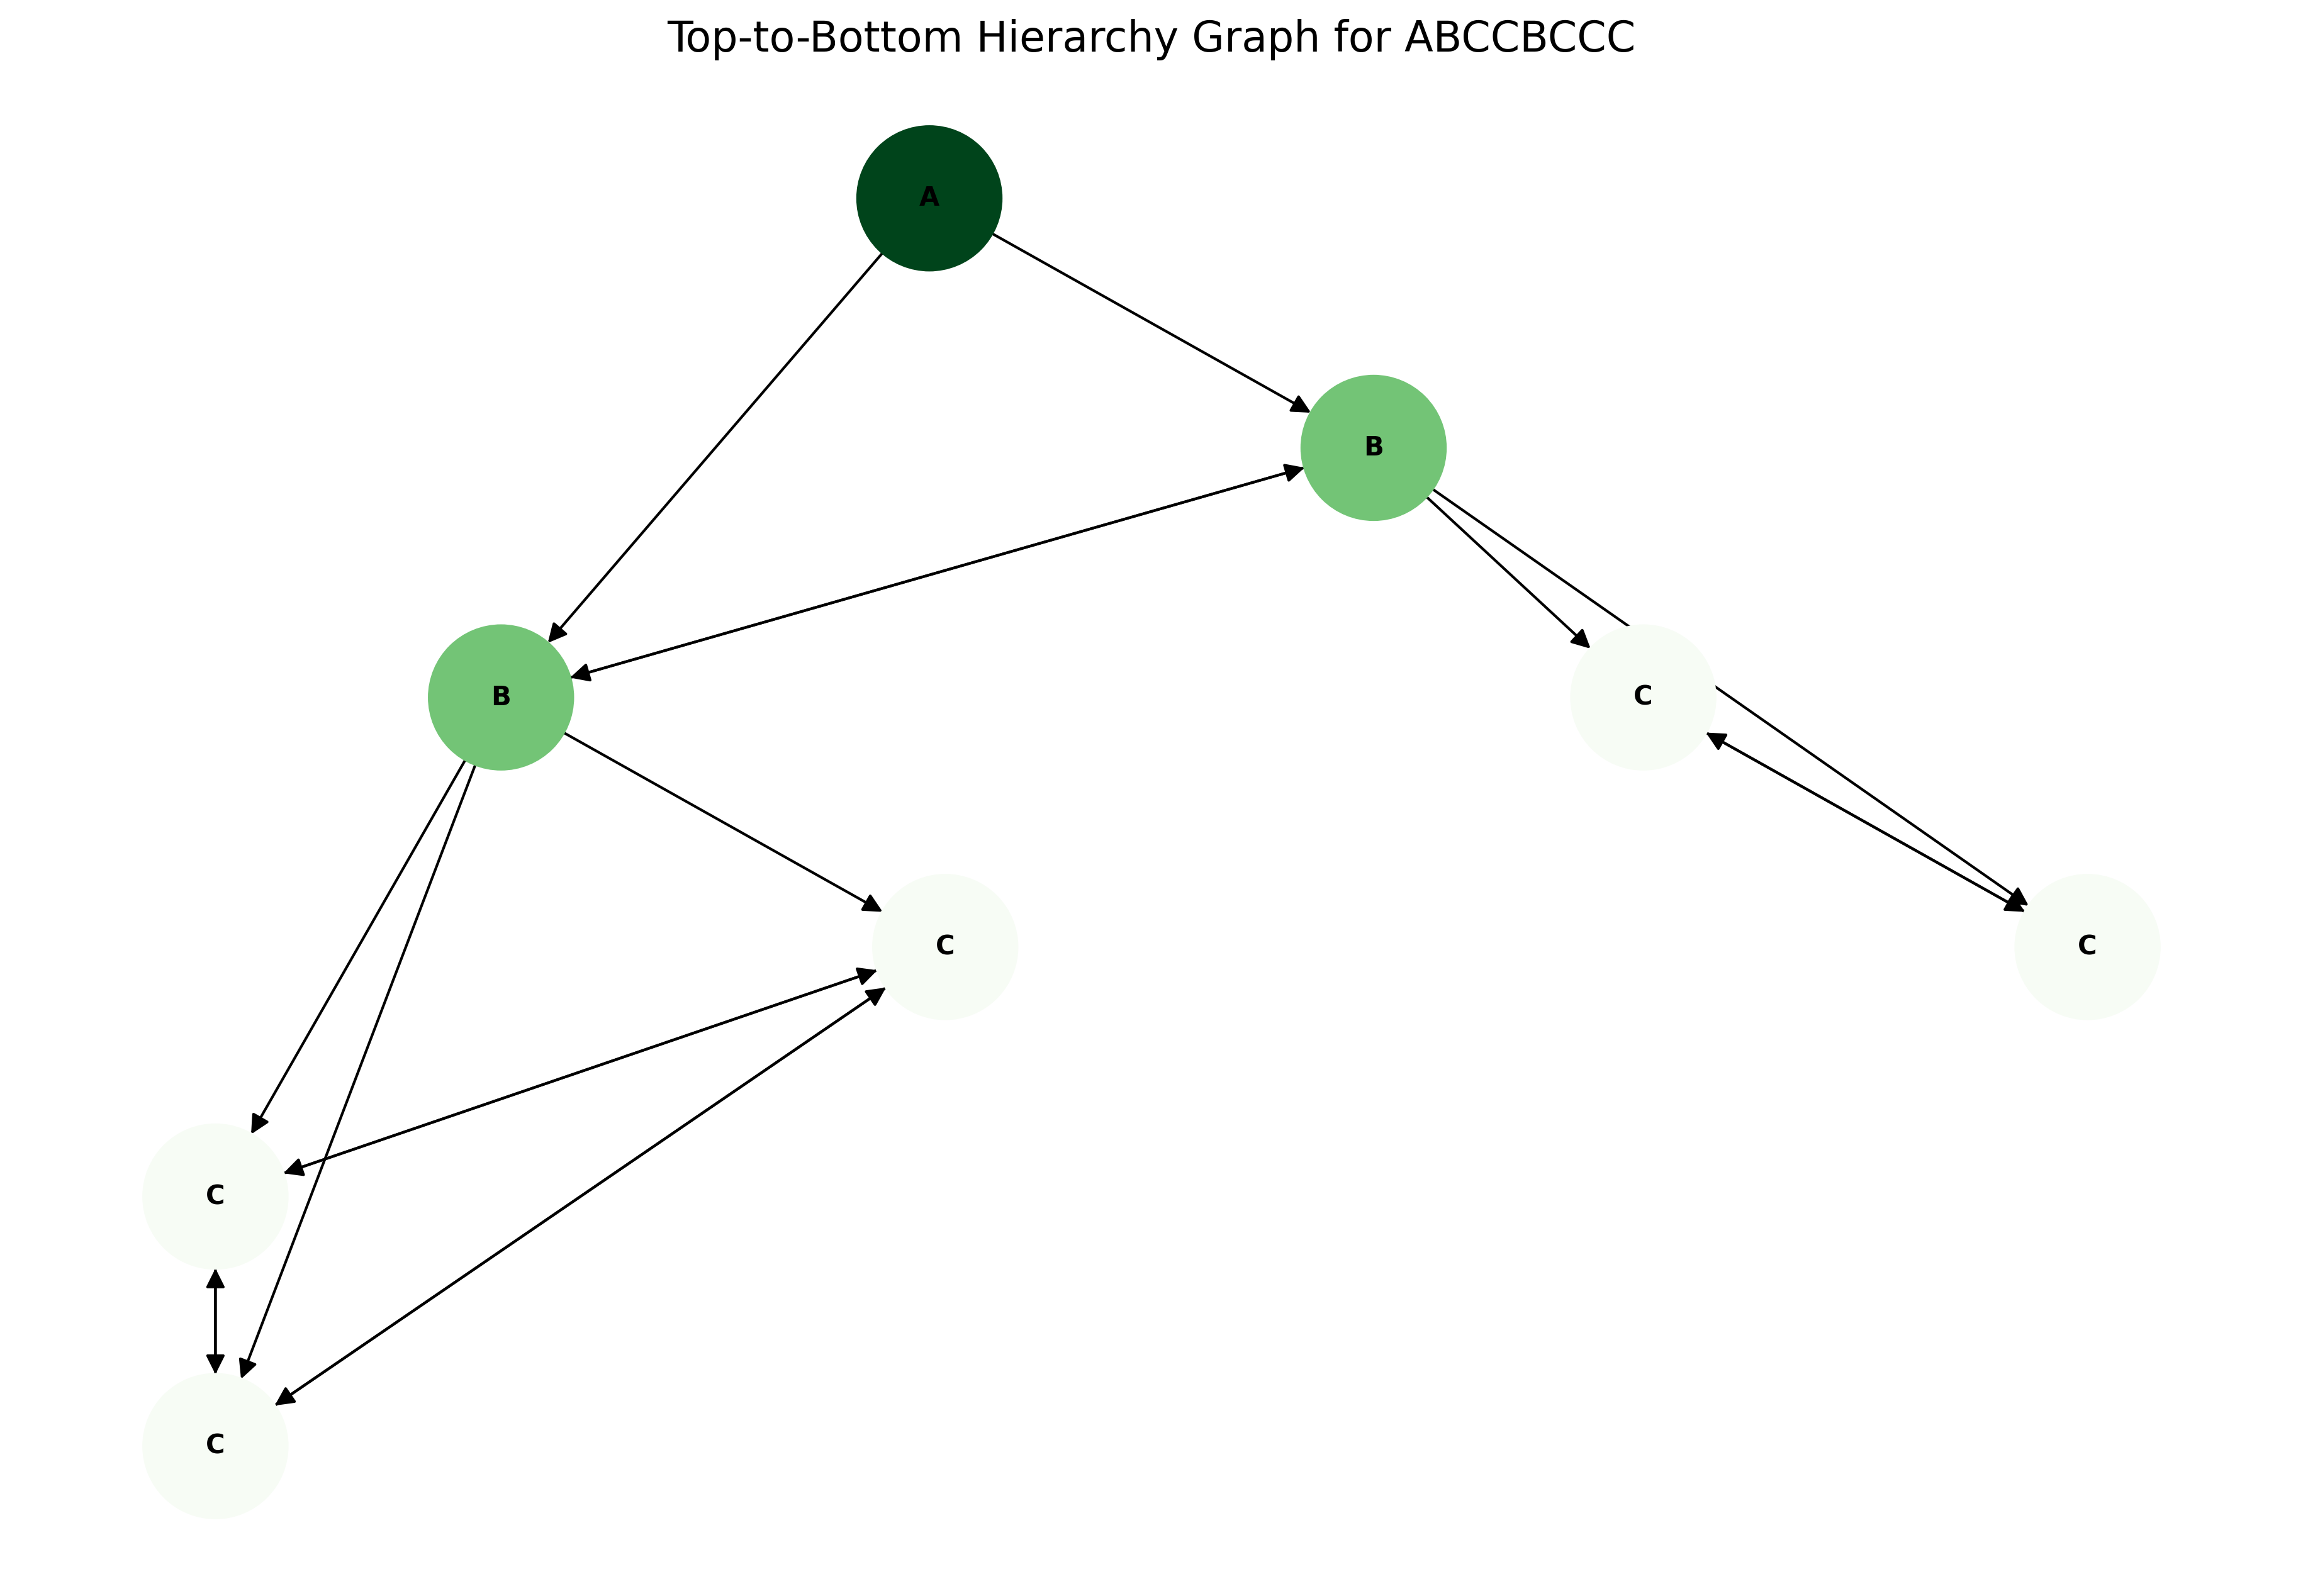
\includegraphics[width=0.8\textwidth]{img/section_methodology/ABCCBCCC.png}
    \caption{A Visualization of the Large "ABCCBCC" Hierarchy}
    \label{fig:large}
\end{figure}

In this test, both the zero-shot AI agent and the "ABCCBCCC" structure will be tasked with solving 200 questions and then checked against the answer key. While this test contains fewer questions than the first one, this is to compensate for the additional computing time due to the complex structure in this version. This test will evaluate whether the deeper hierarchies lead to better accuracy compared to the simpler hierarchies, and how that compares to the added computational intensity.

Through testing with both a simple hierarchy and a complex hierarchy, we will evaluate the practical difference in output between having a multi-agent debate structure, the complexity of the structure, and how the scalability affects the computational intensity.

\subsection{Testing Procedure}
The process the different AI structures followed in answering questions and providing results were done systematically, ensuring structure, consistency, and reproducibility. Each of these tests consists of question selection, execution by the agent, evaluation, and then storing the results.

\subsubsection{Question Selection}
The first part of the experiment is choosing a question for both structures to answer. These questions were sourced from a dataset containing mathematical problems, and also had the correct numerical answer for each question. For Test 1, we randomly selected 1000 questions, and for Test 2, we randomly selected 200 questions. Test 2 contained less questions due to the time complexity of the "ABCCBCCC" structure.

\subsubsection{Agent Execution}
Each question was processed in parallel by both the zero-shot agent and the multi-agent debate system. While the zero-shot agent was only prompted once to generate a response, the multi-agent model processed it in its hierarchical structure. The Prompt Generator Agent structured the problem, the Subordinate Agents independently tried to solve the problem, and the Checker Agent determined whether various answers converged. Until this convergence was achieved, the multi-agent debate continued across multiple rounds. For computational purposes and preventing an infinite loop, the maximum number of debate rounds was capped to 21.

\subsubsection{Evaluation}
Each answer by the AI systems were compared against the true answer provided by the dataset using an automated function. Since the problems were mathematical problems, the responses were parsed to extract only the numerical values, and this was compared against the benchmark answer. If the extracted numerical value was accurate within a tolerance of 1e-6, then it was marked as correct. Otherwise, it was marked incorrect.
The metrics that were tracked are: correct/incorrect responses, response times for both the single agent and the multi-agent system, and the round count for the multi-agent system. These are all necessary metrics to track the accuracy of both systems as well as the computational difference.

\subsubsection{Data Storage}
For structure and reproducibility, the test data was stored in a clear hierarchical format, ensuring easy accessibility to any necessary test data. Each test is stored in its own folder, containing: hierarchy visualization, summary of performance metrics, and stored conversation logs in another folder.

\subsection{Expected Outcomes}
We expect to see trade-offs between the different systems given their unique structures, across accuracy, execution time, and scalability. Accuracy can be expected to increase with the complexity of the system and the number of agents, so we would expect the "ABCCBCCC" multi-agent model to be the most accurate, with the simpler "ABB" structure being second and the zero-shot model being the lowest. As for execution time, the reverse would be true, with the simplest zero-shot model being the fastest and the large hierarchical model being the slowest. As for scalability, we would expect there to be diminishing returns in accuracy compared to computation meaning that the difference in performance would degrade with the depth of the hierarchy.
\section{Result Analysis}
\label{sec:result}

\subsection{Comparative Analysis of Different Topological Structures}
We evaluated the performance of the multi-agent system using two different hierarchical structures: \textit{ABCCBCCC} and \textit{ABB}. The experiments were conducted with both the multi-agent system and a zero-shot agent. Both systems utilized GPT-4o-mini-2024-07-18 and were tested on the GSM8K dataset for the task of solving mathematical word problems. The results are summarized in Table \ref{tab:performance_metrics}. The ABCCBCCC structure consists of eight hierarchical levels, whereas the ABB structure has three levels.


\begin{table}[h]
  \centering
  \caption{Performance for Different Hierarchy Structures}
  \label{tab:performance_metrics}
  \begin{tabular}{l|c|c}
      \hline
      \text{Hierarchy} & \text{ABCCBCCC} & \text{ABB} \\
      \hline
      \text{Total Questions} & 200 & 1000 \\
      \hline
      \text{Accuracy (Zero-Shot Agent)} & 71.5\% & 69.8\% \\
      \hline
      \text{Accuracy (Multi-Agent System)} & \textbf{92.5\%} & 90.0\% \\
      \hline
      \text{Accuracy Improvement} & \textbf{+21.0\%} & +20.2\% \\
      \hline
      \text{Time per Question (Zero-Shot)} & 2.73 sec & 2.93 sec \\
      \hline
      \text{Time per Question (Multi-Agent)} & 68.66 sec & \textbf{22.48 sec} \\
      \hline
      \text{Processing Time Increase} & \(\times 25.15\) & \(\boldsymbol{\times} \mathbf{7.67}\) \\
      \hline
      \text{Efficiency Score (Accuracy / Time)} & 1.35 & \textbf{4.00} \\
      \hline
      \text{Characteristics} & \textbf{Slow, High Accuracy} & \textbf{Balanced} \\
      \hline
  \end{tabular}
\end{table}

The results indicate that the multi-agent system significantly enhances accuracy by 21.0\% and 20.2\% for the ABCCBCCC and ABB structures, respectively. Specifically, the accuracy achieved by the multi-agent system is 92.5\% for the ABCCBCCC structure and 90.0\% for the ABB structure, demonstrating its superiority over the zero-shot agent. Furthermore, the findings suggest that both structural complexity and the number of nodes influence accuracy, with increased complexity and a greater number of nodes leading to improved performance. However, this improvement incurs a computational cost, as the processing time increases by a factor of 25.15 for the ABCCBCCC structure and 7.67 for the ABB structure, highlighting the inherent trade-off between accuracy and computational efficiency. 

To quantitatively assess this trade-off, the efficiency score, defined as the ratio of accuracy to processing time, is introduced. The ABCCBCCC structure achieves an efficiency score of 1.35, indicating a highly accurate but computationally intensive system, whereas the ABB structure attains a score of 4.00, representing a more balanced trade-off. These results suggest that while the ABCCBCCC structure prioritizes accuracy at the expense of efficiency, the ABB structure provides a more optimal balance between accuracy and processing time.

Furthermore, beyond computational efficiency, the financial cost associated with running the multi-agent system must also be considered. In this system, each node hosts multiple agents that iteratively generate responses and engage in debates. As a result, the number of requests to the LLM model increases proportionally with the number of nodes and agents, potentially leading to significantly higher costs.

\subsection{Conversation Analysis}
Through directly looking into the interaction between agents in the hierarchical debate structures, we can gain insights as to how the debate process contributes to the improved accuracy we observed in the experiment statistics. In addition to the debate, it is important to note the contributions of the Prompt Generator and the Checker Agent, which works to break down the problem in a defined way and ensures convergence to a single final answer. This provides structure to the debate process, ensuring consistent results. 

The major advantage of the multi-agent system is its ability to self-correct through peer review, reducing the likelihood of individual errors by AI agents affecting the final results. Even if some or all AI agents may have the wrong answer initially, the debate process allows them to build on their previous attempts and collaborate, guiding them towards converging with the correct answer eventually.

\subsubsection{Example 1: Quick Convergence}
The following is an example of a quick convergence from the ABB hierarchy's conversation history, testing its capability against 1000 questions. The question was the following:

\textit{"Janet’s ducks lay 16 eggs per day. She eats three for breakfast every morning and bakes muffins for her friends every day with four. She sells the remainder at the farmers' market daily for 2 dollars per fresh duck egg. How much in dollars does she make every day at the farmers' market?"}

In this example, both agents correctly calculated that there were 9 eggs left, and 18 dollars in revenue. Since they both arrived at the same conclusion, the Checker Agent recognized the convergence and terminated the debate.

\subsubsection{Example 2: Delayed Convergence}
While oftentimes the AI agents arrive at the same answer in the first round, there are times when they disagree, and a debate takes place until they come to an agreement. The following is an example from the BCC (part of ABCCBCCC) conversation history when tested with 200 questions. The question was:

\textit{"Josh decides to try flipping a house. He buys a house for 80,000 dollars and then puts in 50,000 dollars in repairs. This increased the value of the house by 150 percent. How much profit did he make?"}

While the correct answer was 70,000 dollars, both agents initially arrived at an incorrect answer. Agent 1 incorrectly computed the total expenditure instead of the profit, declaring the answer to be 130,000. Agent 2 incorrectly added the percentage increase rather than multiplying it, declaring 200,000. The Checker Agent detected the disagreement between the two agents, and the debate continued into the next round. In the second round, Agent 1 recognized their misunderstanding by recognizing that the question specifically asked for profit and not the total cost. Meanwhile, Agent 2 also adjusted their answer after seeing Agent 1's reasoning and recognizing that they were supposed to multiply the percentage rather adding it. After this, both agents converged at the correct answer, 70,000 dollars. The Checker Agent validated that both agents came to the same answer, and terminated the debate.

This highlights the importance of the debate system and having multiple agents in arriving to an accurate answer. Even with both agents arriving at the wrong answer initially, they reviewed each other's responses and recognized their own wrongs, ultimately converging on the correct answer. With a zero-shot agent, such debate would have never taken place, and the initial wrong answers would have been considered the final. Such an example indicates that increased debate, with potentially more agents, would further help to increase the accuracy of the answers, although this would require more computational overhead.


\section{Discussion}
\label{sec:discussion}

Our study suggests that incorporating hierarchical depth into the communication topology of LLM agents enhances overall accuracy by enabling multi-level collaboration and introducing redundancy to mitigate errors. While our results do not explicitly demonstrate that a deeper hierarchical communication topology (ABCCBCCC) outperforms a shallower one (ABB) in accuracy, the analysis of conversation history suggests that increased redundancy improves self-correction. This effect may become more pronounced when testing these systems on more complex problem sets. However, redundancy and computational efficiency are inherently trade-offs, and implementing redundancy within a multi-agent debate framework is computationally demanding.

Looking ahead, we propose exploring adaptive optimization methods—such as evolutionary algorithms (e.g., NEAT\cite{stanley:ec02}) or reinforcement learning—to optimize the communication topology to specific problem characteristics, although defining what constitutes a “more optimized” topology remains an open question given the high-dimensional nature of intelligence. In addition, dynamically modifying intrinsic agent properties, such as character or temperature, would promote divergent, out-of-the-box reasoning by diversifying response generation\cite{liang2024encouragingdivergentthinkinglarge}; however, this approach requires regenerating outputs for evaluation within an evolutionary framework, further increasing computational demands.
\section{Conclusion}
\label{sec:conclusion}

This study demonstrates that incorporating a hierarchical communication topologies into a multi-agent debate system enhances accuracy compared to zero-shot reasoning. Furthermore, our analysis suggests that redundancy in communication may strengthen the system’s self-correcting ability, leading to more reliable outcomes.


\newpage

% sections
% \nocite{*}
\bibliographystyle{unsrt}
\bibliography{bib/main}

\newpage
\section{Appendix: Code}

% Define VSCode Light Theme Colors
\definecolor{vscode-bg}{HTML}{FFFFFF}        % Background color (white)
\definecolor{vscode-fg}{HTML}{000000}        % Default text color (black)
\definecolor{vscode-keyword}{HTML}{0000FF}   % Keywords (blue)
\definecolor{vscode-string}{HTML}{A31515}    % Strings (dark red)
\definecolor{vscode-comment}{HTML}{008000}   % Comments (green)
\definecolor{vscode-function}{HTML}{795E26}  % Function names (brownish)
\definecolor{vscode-variable}{HTML}{001080}  % Variables (dark blue)
\definecolor{vscode-number}{HTML}{098658}    % Numbers (greenish)

% Configure listings to mimic VSCode Light Theme
\lstset{
    language=Python,        % Specify the language
    backgroundcolor=\color{vscode-bg}, % Set background color to white
    basicstyle=\ttfamily\small\color{vscode-fg}, % Monospaced normal size font with black text
    commentstyle=\color{vscode-comment}\ttfamily, % Comments in green
    keywordstyle=\color{vscode-keyword}\bfseries, % Keywords in blue and bold
    stringstyle=\color{vscode-string}, % Strings in dark red
    identifierstyle=\color{vscode-variable}, % Variables in dark blue
    numberstyle=\color{gray}, % Line numbers in gray
    breaklines=true,        % Enable line breaking for long lines
    frame=single,           % Add a frame around the code block
    framexleftmargin=5pt,   % Adjust left margin between frame and line numbers
    framexrightmargin=5pt,  % Adjust right margin
    rulecolor=\color{black}, % Set the frame color to black
    numbers=left,           % Display line numbers on the left
    stepnumber=1,           % Number every line
    showstringspaces=false  % Do not visualize spaces in strings
}

\begin{lstlisting}
from autogen import UserProxyAgent, ConversableAgent, GroupChat, GroupChatManager
from autogen.agentchat.contrib.society_of_mind_agent import SocietyOfMindAgent
import datetime
from dotenv import load_dotenv
import json
import matplotlib.pyplot as plt
import networkx as nx
from networkx.drawing.nx_agraph import graphviz_layout
import openai
import os
from pathlib import Path
import re
import sys
import time


# The name of the GPT model to be used in this multi-agent system
gpt_model = "gpt-4o-mini-2024-07-18"

def acquire_oak():
    """
    Attempts to load the OpenAI API key from a `.env` file. If the key
    is not found, the user is prompted to enter it manually.

    Returns:
        str: The OpenAI API key to be used for subsequent calls.
    """
    load_dotenv()  # Load environment variables from .env if present
    api_key = os.getenv("OPENAI_API_KEY")
    if not api_key:
        print(".env File Not Found.")
        # Repeatedly ask user for API key until a non-empty value is provided
        while True:
            try:
                api_key = input("Enter OpenAI API Key Here: ")
                if not api_key:
                    raise ValueError("API Key cannot be empty.")
                break
            except Exception as e:
                print(f"Error: {e}\nPlease enter the API Key again.")
    else:
        print("OpenAI API Key Found!")

    # Set the global OpenAI API key once obtained
    openai.api_key = api_key
    return api_key


def validate_oak():
    """
    Validates that the acquired OpenAI API key is usable by attempting
    to list available models from the OpenAI API. Exits the script if
    validation fails.
    """
    try:
        openai.models.list()
        print("API Key is valid ✅")
    except Exception as e:
        print(f"Error validating API key: {e}")
        sys.exit(1)


def llm_configurator(api_key):
    """
    Constructs a configuration dictionary for the language model,
    containing the model name and the provided API key.

    Args:
        api_key (str): The OpenAI API key to be used.

    Returns:
        dict: A dictionary specifying the model and API key settings.
    """
    return {
        "model": gpt_model,
        "api_key": api_key
    }


def initiate_user_query():
    """
    Prompts the user for a problem or query.

    Returns:
        str: The user-input query string.
    """
    query = input("Please enter your query/problem here: ")
    return query


def get_integer_input(prompt, min_value=None, error_message="Invalid input."):
    """
    Continuously prompts the user for an integer input until a valid value is provided.

    Args:
        prompt (str): The message to display when asking for user input.
        min_value (int, optional): The minimum valid integer value. If provided, any
                                   user input less than or equal to this value is rejected.
        error_message (str, optional): The message to display if validation fails.

    Returns:
        int: The valid integer provided by the user.
    """
    while True:
        try:
            value = int(input(prompt))
            if min_value is not None and value <= min_value:
                print(error_message)
                continue
            return value
        except ValueError:
            print(error_message)


def get_yes_no_input(prompt):
    """
    Prompts the user for a yes/no response (Y/N). Repeats until the user
    enters a valid response.

    Args:
        prompt (str): The question or instruction to show the user.

    Returns:
        bool: True if the user inputs a "yes"-like response, False if "no"-like.
    """
    while True:
        value = input(prompt).strip().lower()
        if value in ['y', 'yes']:
            return True
        elif value in ['n', 'no']:
            return False
        else:
            print("Please enter 'Y' or 'N'.")


def extract_numeric_answer(text):
    """
    Extracts a numeric answer (float) from a string, specifically if the string
    contains a line matching the pattern '#### <number>'.

    Args:
        text (str): The text that potentially contains the numeric answer.

    Returns:
        float or None: The parsed float value if found, otherwise None.
    """
    match = re.search(r"####\s*([\d.]+)", text)
    return float(match.group(1)) if match else None


def evaluate_numeric_answer(system_answer, benchmark_answer, tolerance=1e-6):
    """
    Evaluates whether the multi-agent system's numeric answer matches a benchmark
    numeric answer within a given tolerance.

    The expected format of both answers is: "#### <Numeric Value>"

    Args:
        system_answer (str): The final answer from the multi-agent system.
        benchmark_answer (str): The reference/benchmark answer to check against.
        tolerance (float, optional): Tolerance for floating-point comparison. Default is 1e-6.

    Returns:
        bool: True if the numeric values match within the given tolerance; False otherwise.
    """
    # Extract numeric answers from both system and benchmark
    system_value = extract_numeric_answer(system_answer)
    benchmark_value = extract_numeric_answer(benchmark_answer)

    # If either extraction fails, we cannot evaluate correctly
    if system_value is None or benchmark_value is None:
        print("Error: Could not extract numeric answer from one or both responses.")
        return False

    # Compare the absolute difference to the specified tolerance
    if abs(system_value - benchmark_value) < tolerance:
        return True
    else:
        return False


def parse_subnodes_generic(letters):
    """
    Parses a sub-graph's list of letters into a hierarchical grouping (i.e., generations).

    The main logic is as follows:
      1. Identify the lowest-ranked letter (e.g., 'A' if it exists).
      2. Gather all letters of the next rank (e.g., 'B') until the next occurrence of the lowest-ranked letter.
         This collection becomes "Gen_0" in the output.
      3. For subsequent ranks (B, C, D, ...), gather consecutive letters of the next rank and store those
         in the appropriate "Gen_X" list.

    For example, in the string "ABCCBCCC":
      - 'A' is the lowest letter. You collect 'B' letters that appear after 'A' but before the next 'A'.
      - Then for each 'B', you gather consecutive 'C's, and so on.

    Args:
        letters (list or str): A sequence of letters forming a sub-graph. For instance:
                               ['A', 'B', 'C', 'C', 'B', 'C', 'C'] or "ABCCBCCC".

    Returns:
        dict: A dictionary containing the following keys:
            "nodes" (list): The raw sequence of letters in the sub-graph.
            "Gen_0", "Gen_1", "Gen_2", ... : Lists of "subnode" identifiers extracted from the sequence.
              Each key-value pair corresponds to letters arranged in generations.

        Example return structure:
        {
            "nodes": ["A","B","C","C","B","C","C"],
            "Gen_0": ["ABB1"],
            "Gen_1": ["BCC1", "BCC2"],
            "subnode_counts": { ... }
        }
    """
    # Convert the input to a string if it is a list of letters
    s = letters if isinstance(letters, str) else "".join(letters)
    if not s:
        # If no letters are provided, return an empty structure
        return {"nodes": [], "Gen_0": []}

    # Determine the minimum and maximum letters in the string (e.g., A, B, C, ...)
    min_letter = min(s)
    max_letter = max(s)
    # Convert those letters to numerical "ranks" based on 'A' = 0, 'B' = 1, etc.
    min_rank = ord(min_letter) - ord('A')
    max_rank = ord(max_letter) - ord('A')

    # Prepare a dict to store the final results
    result = {"nodes": list(s)}  # raw structure (the exact letters in the sub-graph)

    # ------------------------------------------------------------------
    # PART A: Handle rank 0 (lowest letter) logic
    # ------------------------------------------------------------------
    letter_r0 = chr(ord('A') + min_rank)       # e.g. 'A' if min_letter is 'A'
    letter_r1 = chr(ord('A') + min_rank + 1)   # e.g. 'B' if the next rank exists

    gen_0_key = f"Gen_{0}"
    result[gen_0_key] = []

    # Gather positions in the string where the rank_0 letter occurs
    positions_of_r0 = [i for i, ch in enumerate(s) if ch == letter_r0]

    if positions_of_r0:
        # Append a sentinel index at the end of the string
        positions_of_r0.append(len(s))

        # For each occurrence of the rank_0 letter (e.g. 'A'), collect
        # consecutive letters of rank_1 (e.g. 'B') until we hit the next 'A'
        for idx in range(len(positions_of_r0) - 1):
            start = positions_of_r0[idx]
            end = positions_of_r0[idx + 1]

            # Count how many letters of the next rank appear between these indices
            B_count = 0
            if min_rank + 1 <= max_rank:
                B_count = sum(1 for j in range(start + 1, end) if s[j] == letter_r1)

            # Construct a subnode string (e.g. "A" + "B"*some_count)
            subnode_str = letter_r0 + (letter_r1 * B_count)

            # Tally how many times this particular subnode string has appeared
            subnode_count = result.get("subnode_counts", {})
            subnode_count[subnode_str] = subnode_count.get(subnode_str, 0) + 1
            # Generate a unique identifier for this subnode
            unique_subnode_id = f"{subnode_str}{subnode_count[subnode_str]}"
            result[gen_0_key].append(unique_subnode_id)
            result["subnode_counts"] = subnode_count

    # For subsequent generations: B -> C, C -> D, etc.
    for i in range(min_rank, max_rank):
        letter_current = chr(ord('A') + i)
        letter_next = chr(ord('A') + i + 1)
        # Skip the rank_0 subnodes (already handled)
        if i == min_rank:
            continue

        # Prepare a new list to store subnodes for this generation
        result_gen_key = f"Gen_{i - min_rank}"
        result[result_gen_key] = []

        # Scan through the string to find letter_current (e.g. 'B'),
        # then gather consecutive letter_next (e.g. 'C') immediately following
        pos = 0
        while pos < len(s):
            if s[pos] == letter_current:
                pos2 = pos + 1
                count_next = 0
                while pos2 < len(s) and s[pos2] == letter_next:
                    count_next += 1
                    pos2 += 1

                if count_next > 0:
                    # Construct e.g. "B" + "C"*count
                    subnode_str = letter_current + (letter_next * count_next)
                    result[result_gen_key].append(subnode_str)

                pos = pos2
            else:
                pos += 1

    return result


def generate_hierarchy_graph(hierarchy_string):
    """
    Creates and saves a NetworkX-directed graph for visualizing the subnode hierarchy
    derived from a given hierarchy string.

    This function:
      1. Splits the hierarchy string by top-level 'A' occurrences (if any).
      2. For each top-level node, calls parse_subnodes_generic() to identify subnodes.
      3. Builds a Directed Graph (nx.DiGraph) where each subnode is linked according to
         a parent-child (and sibling) relationship.
      4. Visualizes the resulting graph with matplotlib, applying a color gradient
         based on the rank of each letter ('A' as rank=0, 'B' as rank=1, etc.).
      5. Saves the resulting graph to "hierarchy_graph.png" in the global output_directory.

    Args:
        hierarchy_string (str): A string that starts with 'A', representing
                                the structure of your multi-agent hierarchy.
                                Example: "ABB" or "ABCCBCCC".

    Raises:
        ValueError: If the hierarchy string does not start with 'A'.

    Returns:
        None. The generated graph image is saved to disk.
    """
    # The hierarchy string must begin with 'A'
    if not hierarchy_string.startswith("A"):
        raise ValueError("The hierarchy string must start with 'A'.")

    # 1. Split the hierarchy string into top-level nodes
    nodes = []
    current_node = []
    for letter in hierarchy_string:
        # Each time we hit an 'A', start a new top-level node
        if letter == "A":
            if current_node:
                nodes.append(current_node)
            current_node = []
        current_node.append(letter)
    if current_node:
        nodes.append(current_node)

    print("============================= HIERARCHY STRUCTURE ==============================")
    print(f"[INFO] Found {len(nodes)} top-level node(s) in the string.")

    # Parse each top-level node into subnode structures
    all_subnodes = []
    for idx, node_letters in enumerate(nodes, start=1):
        print(f"  - Node {idx} has letters: {node_letters}")

        # Parse the subnode structure of this node
        subnode_structure = parse_subnodes_generic(node_letters)
        all_subnodes.append(subnode_structure)

        # Print out any discovered generation keys (e.g., 'Gen_0', 'Gen_1', etc.)
        for gen_key in sorted(k for k in subnode_structure.keys() if k.startswith("Gen_")):
            gen_list = subnode_structure[gen_key]
            if gen_list:
                print(f"    - Node {idx} has {gen_key} subnodes: {gen_list}")
    print("================================================================================\n")

    # ---------------------------------------------------------------------
    # 3. Build a Directed Graph (DiGraph) using a stack-based logic
    # ---------------------------------------------------------------------
    G = nx.DiGraph()
    node_counter = 1
    generation_dict = {}

    # For each top-level node, build sub-graphs by linking letters in a parent-child fashion
    for i, node in enumerate(nodes):
        parent_stack = []
        instance_count = {}
        parent_to_children = {}

        print(f"=== Building Sub-Graph for Top-Level Node {i + 1} ===")

        for letter in node:
            # Track how many times we have seen this letter so far
            instance_count.setdefault(letter, 0)
            instance_count[letter] += 1
            # Create a unique node_id combining letter, instance count, and node_counter
            node_id = f"{letter}_{instance_count[letter]}_{node_counter}"
            G.add_node(node_id, label=letter)

            current_rank_val = ord(letter) - ord('A')

            # Find the correct parent by popping from parent_stack until we find the proper rank
            while parent_stack:
                top_node_id = parent_stack[-1]
                top_label = G.nodes[top_node_id]['label']
                top_rank_val = ord(top_label) - ord('A')
                # If parent is exactly one rank above, we link them
                if top_rank_val == current_rank_val - 1:
                    G.add_edge(top_node_id, node_id)
                    parent_to_children.setdefault(top_node_id, []).append(node_id)
                    generation_dict[node_id] = generation_dict[top_node_id] + 1
                    break
                else:
                    parent_stack.pop()

            # If no valid parent found in the stack, we set its generation to 1
            if not parent_stack:
                generation_dict[node_id] = 1

            # Create sibling edges if multiple children share the same parent
            if parent_stack:
                top_node_id = parent_stack[-1]
                siblings = parent_to_children.get(top_node_id, [])
                for sibling in siblings:
                    if sibling != node_id:
                        G.add_edge(node_id, sibling)
                        G.add_edge(sibling, node_id)

            # Push the current node_id onto the stack
            parent_stack.append(node_id)

        print(f"Finished building sub-graph for Node {i + 1}, node_counter={node_counter}")
        node_counter += 1

    # ---------------------------------------------------------------------
    # 4. Visualize the Graph with color-coding by rank
    # ---------------------------------------------------------------------
    # We assume 'output_directory' is a global variable or defined externally
    # to store output images. The user can customize the color map or dot layout.

    # 1) Compute the rank of each node from 'A'=0, 'B'=1, etc.
    all_ranks = [ord(G.nodes[n]['label']) - ord('A') for n in G.nodes]
    min_rank = min(all_ranks)
    max_rank = max(all_ranks)
    n_ranks = max_rank - min_rank + 1

    # 2) Choose a matplotlib colormap (e.g., Greens)
    cmap = plt.cm.Greens

    # 3) Assign each node a color based on its rank, normalizing to [0..1]
    color_list = []
    for node_id in G.nodes():
        letter = G.nodes[node_id]['label']
        rank_val = ord(letter) - ord('A')
        if n_ranks > 1:
            normalized_val = (rank_val - min_rank) / (n_ranks - 1)
        else:
            normalized_val = 0
        # invert or use directly, e.g., 1 - normalized_val if you want 'A' darkest
        color_list.append(cmap(1 - normalized_val))

    # Use graphviz's 'dot' layout for hierarchical visualization
    plt.figure(figsize=(12, 8))
    pos = graphviz_layout(G, prog="dot")

    # Extract labels from node attributes
    labels = nx.get_node_attributes(G, "label")

    # Draw the graph with relevant parameters
    nx.draw(
        G, pos,
        with_labels=True,
        labels=labels,
        node_size=3000,
        node_color=color_list,
        font_size=10,
        font_weight="bold",
        arrowsize=15
    )

    plt.title(f"Top-to-Bottom Hierarchy Graph for {hierarchy_string}", fontsize=16)

    # Save the graph to a file
    graph_path = output_directory / "hierarchy_graph.png"
    plt.savefig(graph_path, bbox_inches='tight', dpi=300)
    plt.close()
    print(f"Saved hierarchy graph to: {graph_path}\n")


def single_shot_agent(question):
    """
    Creates a zero-shot agent that provides an immediate answer
    in a single response without any debate. This serves as a baseline
    or benchmark agent for comparison with the multi-agent debate system.

    Args:
        question (str): The user-provided question or prompt to be answered.

    Returns:
        str: The raw text response from the zero-shot agent, which should
             include a numeric answer in the format "#### <Answer>" if needed.
    """
    # Create an OpenAI client instance to handle the request
    client = openai.OpenAI()
    # Send a request to the model with system/user messages, specifying the zero-shot approach
    single_shot_agent = client.chat.completions.create(
        messages=[
            {
                "role": "system",
                "content": """
                You are a helpful assistant and a Zero-Shot Agent.\n\n

                Your task is to directly answer the given question in a single response without any further debate or 
                interaction.\n
                You must provide the most accurate answer possible in your first and only attempt.\n\n

                Make sure to include '#### <Answer>' at the end of your response, where <Answer> is the numeric answer, 
                if the problem requires a numeric result.\n
                There can be one, and only one, '#### <Answer>' at the end.\n
                Do not include any commas, apostrophes, or units of measurement in the numerical answer.\n
                Ensure that your final answer is actually what is being required, rather than an intermediate calculation!\n
                Do not provide explanations beyond the final answer.
                """
            },
            {
                "role": "user",
                "content": f"Question: {question}"
            }
        ],
        model=gpt_model
    )
    # Extract the text of the response
    single_agent_answer = single_shot_agent.choices[0].message.content
    return single_agent_answer


def spawn_user_interface(llm_config):
    """
    Creates a user-facing agent (UserProxyAgent) that
    initiates conversations with the hierarchy.

    Args:
        llm_config (dict): The language model configuration (e.g. model name, API key).

    Returns:
        UserProxyAgent: The agent that represents the user side of the conversation,
                        forwarding user queries to the system.
    """
    user_interface = UserProxyAgent(
        name="User_Interface",
        # This function checks for the word 'TERMINATE' in the content to decide if it should stop
        is_termination_msg=lambda x: x.get("content", "").find("TERMINATE") >= 0,
        human_input_mode="NEVER",  # No interactive human input during the script
        code_execution_config=False,  # No code execution permission
        llm_config=llm_config,
    )
    return user_interface


def spawn_prompt_generator(llm_config, gen_name, subnode):
    """
    Spawns an agent whose sole purpose is to generate a structured prompt
    based on the user problem statement, without actually solving it.

    Args:
        llm_config (dict): Configuration dictionary for the LLM.
        gen_name (str): The generation label (e.g., 'Gen_0').
        subnode (str): The identifier for this subnode (e.g., 'ABB1').

    Returns:
        ConversableAgent: An agent that will produce a prompt summarizing the problem
                          and its requirements, instructing other agents to solve it.
    """
    prompt_generator = ConversableAgent(
        name="Prompt_Generator",
        # The following system_message instructs the agent on how to create prompts
        system_message=(f"""
            You are a prompt generator designed to assist other language model agents in solving problems accurately.\n
            In this multi-agent system, you have been assigned to a particular section, called a subnode.\n
            You are a member of subnode '{subnode}', belonging to the generation '{gen_name}'.\n\n

            Given a user-provided problem statement, perform the following tasks without attempting to solve the problem.\n\n

            Here are your instructions:\n
            0. **YOU MUST NEVER SOLVE THE PROBLEM**\n
            1. **Identify the Category:** Determine the category or subject of the problem (e.g., Mathematics, Science, 
            Language Arts).**\n
            2. **Summarize the Problem:** Provide a summary of the problem, highlighting key information and relevant 
            data for solving it.**\n
            3. **Specify Requirements:** Outline what is needed to solve the problem. The agents must be able to solve 
            the problem based on the information that you give them, so it must be complete.**\n
            4. **Tell agents that they need to solve the problem.**\n
            5. **If the debate continues because convergence is not reached, simply repeat the original prompt.**\n
            6. You are NEVER allowed to say 'TERMINATE'.\n\n

            Generate the prompt in English following this structure:\n\n

            ---\n"
            **Category:** [Determined Category]\n\n
            **Problem Summary:** [Summary]\n\n
            **Requirements:** [List of Requirements]\n
            **Instructions to Agents:** [Clear instructions to solve the problem]
            ---
        """),
        is_termination_msg=lambda x: x.get("content", "").find("TERMINATE") >= 0,
        code_execution_config=False,
        llm_config=llm_config,
    )
    return prompt_generator


def spawn_counter(llm_config, gen_name, subnode):
    """
    Spawns an agent that simply counts the number of debate rounds until 'TERMINATE' occurs.

    Args:
        llm_config (dict): The LLM configuration.
        gen_name (str): Generation label (e.g., 'Gen_0', 'Gen_1').
        subnode (str): Identifier for this subnode.

    Returns:
        ConversableAgent: An agent that will output "Round X" each time it speaks,
                          incrementing the round count each time, until termination.
    """
    counter = ConversableAgent(
        name="Counter",
        # The system message explains the agent’s role in counting debate rounds
        system_message=(
            "You are a helpful assistant. You are one of the agents of a multi-agent debate system.\n\n"
            "In this multi-agent system, you have been assigned to a particular section, called a subnode.\n"
            f"You are a member of subnode '{subnode}', belonging to the generation '{gen_name}'.\n\n"
            "A debate is composed of a series of responses by agents.\n"
            "A debate round begins with the response by the first agent and ends with the evaluation by the Checker agent.\n"
            "You are going to count the number of debate rounds.\n"
            "If you do not see any response yet, then it is the beginning of the first round, labelled Round 1.\n\n"
            "**Your output must follow the following format: 'Round <<round_number>>'**\n"
            "**Do not restart at Round 1 unless it's a new problem.**\n"
            "**Stop counting when 'TERMINATE' is detected.**\n"
            "**Do not answer the prompt by the user. Your sole job is counting rounds, following the instructions above.**"
        ),
        llm_config=llm_config
    )
    return counter


def spawn_subordinate_agents(llm_config, gen_name, subnode, idx_sub, agent_letter):
    """
    Spawns subordinate agents that attempt to solve the problem after receiving the prompt.
    They can revise their answers in subsequent rounds based on peer responses.

    Args:
        llm_config (dict): The LLM configuration to use for this agent.
        gen_name (str): The generation name, e.g. 'Gen_0'.
        subnode (str): The subnode identifier (e.g., 'ABB1').
        idx_sub (int): Numerical index for this subordinate agent (e.g. 1, 2, etc.).
        agent_letter (str): A single letter that differentiates subordinate agents (e.g. 'B' or 'C').

    Returns:
        ConversableAgent: A subordinate agent that will produce its own solution in Round 1
                          and refine it in further rounds after reviewing others' solutions.
    """
    agent = ConversableAgent(
        # Construct a name like "Subordinate_Agent_B1_Gen_0_Subnode_ABB1"
        name=f"Subordinate_Agent_{agent_letter}{idx_sub}_{gen_name}_Subnode_{subnode}",
        system_message=(f"""
            You are a helpful assistant. You are one of the agents of a multi-agent debate system.\n\n

            In this multi-agent system, you have been assigned to a particular section, called a subnode.\n
            The subnode works like a group chat. You will be chatting with the other agents of your kind.\n\n

            You are a Subordinate member of subnode '{subnode}', belonging to the generation '{gen_name}'.\n\n

            Given a structured prompt provided by the Prompt Generator agent, please do the following:\n"
                1. In Round 1, do NOT look at or acknowledge previous Agents' responses. Solve the problem INDEPENDENTLY,
                 ALWAYS providing your own explanation because the user needs to see your reasoning;\n
                2. IF, AND ONLY IF, you are in Round 2 or later, review the responses of the other Subordinate Agents and
                provide your own explanation based on their contributions;\n
                3. From Round 2 onwards, refine your own response until the Checker Agent says 'TERMINATE'.\n\n

            A debate is composed of a series of responses by agents.\n
            A debate round begins with the response by the first agent and ends with the evaluation by the Checker agent.\n
            The round ends after all agents have responded.\n
            Please NEVER count the Rounds. There is a specific Counter Agent for that purpose.\n\n

            Make sure to include '#### <Answer>' at the end of your response, where <Answer> is the numeric answer, 
            if the problem requires a numeric result. Before that, make sure to always provide your explanation.\n
            There can be one, and only one, '#### <Answer>' at the end.\n
            Do not include any commas, apostrophes, or units of measurement in the numerical answer.\n
            Ensure that what you put in '#### <Answer>' is actually what is being required, rather than an intermediate number!\n
            """),
        is_termination_msg=lambda x: x.get("content", "").find("TERMINATE") >= 0,
        code_execution_config=False,
        llm_config=llm_config,
        description=("""
                    Subordinate Agent tasked with:\n
                    1. Generating a response to find a solution to the problem provided by the user;\n
                    2. Reviewing other Subordinate Agents' responses only from Round 2 onwards;\n
                    3. Refining its own response in future rounds of debate based on the contributions by the other
                    Subordinate Agents, until the Checker Agent says 'TERMINATE'.
                    """)
    )
    return agent


def spawn_checker(llm_config, gen_name, subnode):
    """
    Spawns the Checker agent for a given subnode. This agent evaluates all subordinate agents’
    responses and decides if they converge (agree on the same answer). If they do, it outputs 'TERMINATE';
    otherwise, it outputs 'CONTINUE'.

    Args:
        llm_config (dict): The LLM configuration.
        gen_name (str): The generation name of the subnode (e.g. 'Gen_0').
        subnode (str): The identifier for the subnode (e.g., 'ABB1').

    Returns:
        ConversableAgent: The Checker agent that can end the debate or request more rounds.
    """
    checker = ConversableAgent(
        name="Checker",
        system_message=(f"""
        You are a helpful assistant. You are one of the agents of a multi-agent debate system.\n\n

        In this multi-agent system, you have been assigned to a particular section, called a subnode.\n
        The subnode works like a group chat. However, you do not participate to the discussion.\n\n

        You are a member of subnode '{subnode}', belonging to the generation '{gen_name}'.\n\n

        You are tasked with evaluating the responses generated by multiple LLM Agents within your subnode.\n
        Those agents will be collaborating to solve the same problem.\n
        Your job is to evaluate their responses and determine if they have reached a consensus.\n
        If the agents provide responses that are similar in meaning and consistent, then you must reply 'TERMINATE' to end the debate.\n
        Otherwise, reply 'CONTINUE' to allow another discussion round.
        """),
        is_termination_msg=lambda x: x.get("content", "").find("TERMINATE") >= 0,
        code_execution_config=False,
        llm_config=llm_config,
    )
    return checker


def spawn_subnode_group_chat(all_agents):
    """
    Creates a GroupChat instance for a given subnode, incorporating:
      - A Chat Manager
      - Prompt Generator
      - Counter
      - Subordinate Agents
      - Checker Agent

    Args:
        all_agents (list): A list of agent objects (ConversableAgent, etc.) that will participate in the subnode chat.

    Returns:
        GroupChat: An object that orchestrates multi-turn conversations among the given agents.
    """
    # We specify the maximum number of rounds to avoid infinite loops.
    # The speaker_selection_method ensures that each agent gets to speak in a round-robin order.
    subnode_group_chat = GroupChat(
        agents=all_agents,  # Agents include Chat_Manager, Prompt_Generator, Counter, Subordinate Agents, and Checker
        messages=[],
        max_round=21,  # Some reasonably large limit; can be tuned or replaced dynamically
        speaker_selection_method="round_robin",
    )
    return subnode_group_chat


def spawn_chat_manager(subnode_group_chat, llm_config, gen_name, subnode, chat_manager_letter, subordinates_letters):
    """
    Creates and configures a GroupChatManager for the specified subnode, which controls
    how the conversation flows among the agents (Prompt Generator, Counter, Subordinates, Checker).

    Args:
        subnode_group_chat (GroupChat): The GroupChat object that contains the relevant agents for this subnode.
        llm_config (dict): The language model configuration.
        gen_name (str): The generation name for the subnode (e.g., 'Gen_0').
        subnode (str): The subnode identifier (e.g., 'ABB1').
        chat_manager_letter (str): A single letter identifying the chat manager (e.g., 'A').
        subordinates_letters (list): Letters that identify the subordinate agents (e.g., ['B', 'B']).

    Returns:
        GroupChatManager: An object that orchestrates the order of speaker turns and can detect termination events.
    """
    chat_manager = GroupChatManager(
        groupchat=subnode_group_chat,
        name=f"Chat_Manager_{chat_manager_letter}_{gen_name}_Subnode_{subnode}",
        system_message=(f"""
        You are managing a Group Chat where Agents must discuss and collaborate to find a solution to a problem provided 
        by the user and structured into a prompt by a prompt generator.\n\n

        The order of speakers in the Group Chat **must** be the following and cannot be altered:\n
        1. **Prompt Generator** (only in the very first round).\n
        2. **Counter Agent**.\n
        3. **All subordinate agents** (ordered alphabetically).\n
        4. **Checker Agent** (ONLY AFTER all working agents have responded).\n
        5. If convergence is achieved, you must also end the debate by simply saying 'TERMINATE'..\n
           Otherwise, start again from step 1 (Prompt Generator).\n\n

        **You must strictly enforce this order and ensure no agent speaks out of turn.**

        Your responsibilities are the following:\n
        1. Ensure that each Agent produces a response.\n
        2. Strictly enforce the speakers order and ensure no agent speaks out of turn.\n
        3. If the Checker Agent does not detect convergence and says 'CONTINUE', allow another round of debate.\n
        In such a case, ensure that the Agents update their responses based on the responses from the previous rounds 
        of debate.\n
        4. If the Checker agents detects convergence and says 'TERMINATE', terminate the debate by saying 'TERMINATE'.
        """),
        is_termination_msg=lambda x: x.get("content", "").find("TERMINATE") >= 0,
        llm_config=llm_config,
    )
    # Print a quick info message to identify the chat manager and subordinates
    print(
        f"  -> Manager of the GroupChat: '{chat_manager_letter}', "
        f"Subordinates: {list(subordinates_letters)}.\n"
    )
    return chat_manager


def spawn_hierarchy_manager(
        chat_manager, llm_config, gen_name, subnode, chat_manager_letter, user_query
):
    """
    Spawns a Hierarchy Manager (SocietyOfMindAgent) responsible for handing off the user query
    to the subnode-level Chat Manager. The Hierarchy Manager enforces a one-time pass of the user
    query to avoid restarting the subnode multiple times.

    Args:
        chat_manager (GroupChatManager): The GroupChatManager that orchestrates the subnode.
        llm_config (dict): Configuration dict with model and API key.
        gen_name (str): Generation label (e.g. 'Gen_0').
        subnode (str): Subnode identifier (e.g. 'ABB1').
        chat_manager_letter (str): Letter identifying this chat manager.
        user_query (str): The original user query/problem statement.

    Returns:
        SocietyOfMindAgent: The hierarchy manager that can initiate a single pass of the subnode chat.
    """
    hierarchy_manager = SocietyOfMindAgent(
        name=f"Hierarchy_Manager_{chat_manager_letter}_{gen_name}_Subnode_{subnode}",
        chat_manager=chat_manager,
        is_termination_msg=lambda x: x.get("content", "").find("TERMINATE") >= 0,
        code_execution_config=False,
        llm_config=llm_config,
    )

    # A private boolean to indicate if the subnode chat has already run
    hierarchy_manager._subnode_done = False

    def process_handoff(*args, **kwargs):
        """
        Initiates the subnode chat exactly once by passing the user query to the chat manager.
        If run again, it would still pass the query, but in your final code you might
        guard against re-initiation if you only want it to run once.
        """
        print(f"Hierarchy_Manager_{chat_manager_letter} passing original user query to subnode {subnode}.")
        return chat_manager.initiate_chat(chat_manager, message=user_query, clear_history=False)

    # Overwrite the default .initiate_chat method with the custom process_handoff
    hierarchy_manager.initiate_chat = process_handoff

    return hierarchy_manager


def llm_parser(aggregated_answer):
    """
    Uses an additional LLM-based parser to extract the final numeric answer from
    a possibly verbose response, returning it in the standardized format '#### <Answer>'.

    Args:
        aggregated_answer (str): The final combined answer from a multi-agent debate.

    Returns:
        str: A parsed string of the form "#### <numeric_value>", with no extra text.
    """
    client = openai.OpenAI()
    parser = client.chat.completions.create(
        messages=[
            {
                "role": "system",
                "content": """
                You are an LLM Parser. Your job is to parse the final answer from other LLM agents.\n
                You are tasked with summarizing the answer in a single number, without any extra words.\n\n

                Your response should just contain a number WITHOUT any commas, apostrophes, or units of measurement.\n
                Format:\n
                #### <<Numeric Answer>>\n\
                """,
            },
            {
                "role": "user",
                "content": f"Answer: {aggregated_answer}"
            }
        ],
        model=gpt_model
    )
    parsed_answer = parser.choices[0].message.content
    return parsed_answer


def create_group_chat(llm_config, gen_name, subnode):
    """
    Initializes and returns the subnode group chat by creating and collecting:
      - A Prompt Generator agent,
      - A Counter agent,
      - Subordinate agents,
      - A Checker agent,
      - A Chat Manager to orchestrate the conversation.

    Args:
        llm_config (dict): The configuration for the LLM.
        gen_name (str): The generation name, e.g. 'Gen_0'.
        subnode (str): A string like 'ABB1' that identifies the subnode.

    Returns:
        GroupChatManager: The chat manager that coordinates all agents for this subnode.
    """
    print(f"\nCreating GroupChat for Subnode: {subnode}")

    # List to hold all agent instances for this subnode
    all_agents = []

    # Create the Prompt Generator (which never solves, only outlines the problem)
    prompt_generator = spawn_prompt_generator(llm_config, gen_name, subnode)
    all_agents.append(prompt_generator)

    # Create the Counter agent
    counter = spawn_counter(llm_config, gen_name, subnode)
    all_agents.append(counter)

    # The first letter in subnode indicates the Chat Manager (e.g. 'A')
    # The rest are subordinate letters (e.g. 'B', 'B') or similar
    chat_manager_letter = subnode[0]
    subordinates_letters = [ch for ch in subnode[1:] if ch.isalpha()]  # Only letters

    # Create subordinate agents (e.g. 'B1', 'B2', etc.)
    working_agents = []
    for idx_sub, agent_letter in enumerate(subordinates_letters, start=1):
        agent = spawn_subordinate_agents(llm_config, gen_name, subnode, idx_sub, agent_letter)
        working_agents.append(agent)

    # Add all subordinate agents to the list
    all_agents.extend(working_agents)

    # Spawn the Checker agent and add to the list
    checker = spawn_checker(llm_config, gen_name, subnode)
    all_agents.append(checker)

    # Create the subnode group chat with all these agents
    subnode_group_chat = spawn_subnode_group_chat(all_agents)

    # Create and return the chat manager for this subnode
    chat_manager = spawn_chat_manager(
        subnode_group_chat, llm_config, gen_name, subnode, chat_manager_letter, subordinates_letters
    )

    return chat_manager


if __name__ == "__main__":

    """
    Main entry point for the multi-agent system execution. This section handles:

    1. API Key retrieval and validation.
    2. User choice of hierarchy string (default or custom).
    3. User choice of using a JSON file with math problems or a custom query.
    4. Setup of the multi-agent framework, including:
        - Parsing of the hierarchy string into subnodes.
        - Generating and saving a hierarchy graph visualization.
        - Spawning Zero-Shot and Multi-Agent systems to answer the question(s).
    5. Orchestrating the final output:
        - Tracking how many questions were correctly answered by Zero-Shot vs Multi-Agent systems.
        - Printing a summary of results and conversation histories.
    """

    # Step 1: Configuration and API Setup
    print("===== Welcome to the Multi-Agent System =====\n")
    api_key = acquire_oak()  # Retrieve API key from .env or user prompt
    validate_oak()  # Validate the acquired API key
    llm_config = llm_configurator(api_key)  # Create a dict with model and API key settings

    # Step 2: Prompt for the Hierarchy String using get_yes_no_input
    if get_yes_no_input("Do you want to use the default hierarchy string 'ABB'? (Y/N): "):
        hierarchy_string = "ABB"
        print(f"Using default hierarchy string: {hierarchy_string}")
    else:
        # Let the user enter a custom hierarchy string, ensuring it starts with 'A'
        hierarchy_string = input("Enter your custom hierarchy string (e.g., ABCCBCCC): ").strip().upper()
        while not hierarchy_string.startswith("A"):
            print("Error: The hierarchy string must start with 'A'.")
            hierarchy_string = input("Enter your custom hierarchy string (e.g., ABCCBCCC): ").strip().upper()
        print(f"Using custom hierarchy string: {hierarchy_string}")

    # Create a timestamped output directory for logs/results
    timestamp = datetime.datetime.now().strftime("%m-%d-%Y_%H-%M-%S")
    output_directory = Path(f"output/{timestamp}")
    output_directory.mkdir(parents=True, exist_ok=True)

    # Step 3: Prompt whether to use the JSON file with math problems or a custom query
    use_json = get_yes_no_input(
        "Do you want to use the JSON file with math problems instead of a custom query? (Y/N): ")
    if use_json:
        # Attempt to open and parse the JSON file containing problems
        try:
            with open("problem_sets.jsonl", "r", encoding="utf-8") as f:
                # Each line in the file is assumed to be a valid JSON object
                data = [json.loads(line) for line in f]
        except FileNotFoundError:
            print('File not found: "problem_sets.jsonl" does not exist in the current directory.')
            sys.exit(1)

        # Extract questions and answers from the JSON lines
        questions = [item["question"] for item in data]
        answers = [item["answer"] for item in data]

        # Ask the user how many questions to process from the loaded file
        num_questions = get_integer_input(
            "How many questions do you want the multi-agent framework to solve? ",
            min_value=0, error_message="The number of questions must be more than 0."
        )
        questions = questions[:num_questions]
        answers = answers[:num_questions]
    else:
        # Custom user query mode if not using the JSON file
        user_query = initiate_user_query()  # Prompt user for a custom question
        questions = [user_query]  # Wrap it into a list for uniform processing
        answers = [None]  # No benchmark answer in custom mode

    # Step 4: Parse the Hierarchy
    print(f"\nParsing the Hierarchy String '{hierarchy_string}'")
    subnode_structure = parse_subnodes_generic(hierarchy_string)

    # Step 5: Visualize the hierarchy (saves the output graph to disk)
    print("Generating the hierarchy graph for visualization...\n")
    generate_hierarchy_graph(hierarchy_string)

    # Step 6: Identify and sort generations in descending order (e.g. Gen_1, Gen_0)
    gens = sorted([k for k in subnode_structure if k.startswith("Gen_")], reverse=True)
    print(f"Generations found (highest first): {gens}")

    # Step 7: Initialize data structures for the multi-agent system
    final_subnode_answers = {}  # e.g. { "BCC": "...", "ABB1": "...", ... }
    manager_to_subnodes = {}  # e.g. { "A": ["ABB1"], "B": ["BCC", "BCCC"], ... }

    # The user-facing agent who interacts with the top-level aggregator (Supreme_Hierarchy)
    user_interface = spawn_user_interface(llm_config)
    chat_managers = {}  # Will hold chat managers for each subnode
    hierarchy_managers = {}  # Will hold hierarchy managers for each subnode

    # If you want to limit the top-level rounds (like if you have 3 subnodes total):
    number_of_subnodes = 1

    # Initialize containers for Zero-Shot vs Multi-Agent answers and evaluation
    parsed_single_agent_answers_list = []
    parsed_multi_agent_answers_list = []

    correct_count_single_agent = 0
    incorrect_count_single_agent = 0

    correct_count_multi_agent = 0
    incorrect_count_multi_agent = 0

    conversation_history_single_agent = []
    conversation_history_multi_agent = {}

    single_shot_durations = []
    multi_agent_durations = []

    # Outer loop: iterate over each question in the list
    for k in range(len(questions)):
        print("\n" + "=" * 80)
        print(f"QUESTION {k + 1}:")
        print("=" * 80)

        question = questions[k]
        benchmark_answer = answers[k] if answers[k] is not None else None

        # --------------------------- Zero-Shot Agent Flow ---------------------------
        start_single_shot = time.time()

        # Obtain zero-shot answer and parse out the numeric portion
        single_agent_answer = single_shot_agent(question)
        parsed_single_agent_answer = llm_parser(single_agent_answer)
        parsed_single_agent_answers_list.append(parsed_single_agent_answer)

        end_single_shot = time.time()
        single_shot_duration = end_single_shot - start_single_shot
        single_shot_durations.append(single_shot_duration)

        # Print zero-shot results
        print(f"Zero-Shot Agent Answer to question {k + 1}: {single_agent_answer}\n")
        print(f"Parsed Zero-Shot Answer: {parsed_single_agent_answer}")
        print(f"Zero-Shot Agent Time: {single_shot_duration:.4f} seconds")

        # Log zero-shot conversation
        conversation_history_single_agent.append({
            "Question": question,
            "True Solution": f"#### {answers[k]}" if answers[k] is not None else "N/A",
            "Zero-Shot Agent Response": single_agent_answer,
            "Parsed Zero-Shot Answer": parsed_single_agent_answer,
            "Zero-Shot Duration (s)": single_shot_duration
        })

        # Evaluate zero-shot answer if we have a benchmark
        if benchmark_answer is not None:
            if evaluate_numeric_answer(parsed_single_agent_answer, benchmark_answer):
                print("Zero-Shot Agent Evaluation: ✅ The answer matches the benchmark answer. Good job!")
                correct_count_single_agent += 1
            else:
                print("Zero-Shot Agent Evaluation: ❌ The answer does NOT match the benchmark answer.")
                incorrect_count_single_agent += 1

        # --------------------------- Multi-Agent Flow ---------------------------
        start_multi_agent = time.time()

        # For each generation (in descending order), create subnode chat managers and hierarchy managers
        for gen_name in gens:
            subnodes = subnode_structure[gen_name]
            if not subnodes:
                continue

            print(f"\n--- Processing {gen_name} subnodes: {subnodes}")
            for subnode in subnodes:
                # Create a manager for this subnode
                chat_managers[subnode] = create_group_chat(llm_config, gen_name, subnode)

                # Map the chat manager letter to this subnode (for reference if needed)
                chat_manager_letter = subnode[0]
                if chat_manager_letter not in manager_to_subnodes:
                    manager_to_subnodes[chat_manager_letter] = []
                manager_to_subnodes[chat_manager_letter].append(subnode)

                # Create a hierarchy manager that feeds user_query into the subnode chat
                hierarchy_managers[subnode] = spawn_hierarchy_manager(
                    chat_manager=chat_managers[subnode],
                    llm_config=llm_config,
                    gen_name=gen_name,
                    subnode=subnode,
                    chat_manager_letter=subnode[0],
                    user_query=question
                )

                # Initialize conversation logs for that subnode if not already present
                if subnode not in conversation_history_multi_agent:
                    conversation_history_multi_agent[subnode] = []

        # Step 8: Create the Supreme Society of Minds that includes the user interface + all hierarchy managers
        hierarchy_managers_values = hierarchy_managers.values()
        hierarchy_managers_list = list(hierarchy_managers_values)
        hierarchy_managers_list.append(user_interface)

        # Build the top-level GroupChat with all the hierarchy managers + user interface
        hierarchies_group_chat = GroupChat(
            agents=hierarchy_managers_list,
            messages=[],
            max_round=number_of_subnodes + 1,  # e.g. if you have 3 subnodes
            speaker_selection_method="round_robin",
        )

        # A manager to orchestrate the top-level group chat, deciding if/when to terminate
        hierarchies_group_chat_manager = GroupChatManager(
            groupchat=hierarchies_group_chat,
            name="Hierarchies_Group_Chat_Manager",
            system_message="""
            You have been assigned the following tasks:
            Step 1. Ensure that all agents generate responses.
            Step 2. Evaluate whether the responses converge in similarity or not.
            Step 3. If they do: 
               - Aggregate the responses into a single one, 
               - Send it to the User_Interface,
               - **Add 'TERMINATE'** at the end to end the entire conversation.
            If they do not converge, start again from Step 1.

            You summarize the answer in a simple single sentence ...
            """,
            is_termination_msg=lambda x: x.get("content", "").find("TERMINATE") >= 0,
            llm_config=llm_config,
        )

        # Create the supreme aggregator (SocietyOfMindAgent) for top-level coordination
        supreme_hierarchy = SocietyOfMindAgent(
            chat_manager=hierarchies_group_chat_manager,
            name="Supreme_Hierarchy",
            code_execution_config=False,
            llm_config=llm_config,
        )

        # The user interface initiates the chat with the Supreme Hierarchy using the question
        chat_result = user_interface.initiate_chat(
            supreme_hierarchy,
            message=questions[k],
        )

        # Retrieve the final aggregated multi-agent answer from the Supreme Hierarchy
        multi_agent_answer = chat_result.chat_history[0]["content"]
        parsed_multi_agent_answer = llm_parser(multi_agent_answer)
        parsed_multi_agent_answers_list.append(parsed_multi_agent_answer)

        end_multi_agent = time.time()
        multi_agent_duration = end_multi_agent - start_multi_agent
        multi_agent_durations.append(multi_agent_duration)

        # Print multi-agent results
        print(f"Multi-Agent Answer: {multi_agent_answer}\n")
        print(f"Parsed Multi-Agent Answer: {parsed_multi_agent_answer}")
        print(f"Multi-Agent System Time: {multi_agent_duration:.4f} seconds")

        # Evaluate multi-agent answer if we have a benchmark
        if benchmark_answer is not None:
            if evaluate_numeric_answer(parsed_multi_agent_answer, benchmark_answer):
                print("Multi-Agent Evaluation: ✅ The system's answer matches the benchmark answer. Good job!")
                correct_count_multi_agent += 1
            else:
                print("Multi-Agent Evaluation: ❌ The system's answer does NOT match the benchmark answer.")
                incorrect_count_multi_agent += 1

        # Save the conversation history for each subnode
        for subnode, chat_manager in chat_managers.items():
            chat_history = chat_manager.groupchat.messages if hasattr(chat_manager, "groupchat") else []
            conversation_history_multi_agent[subnode].append({
                "Question": question,
                "True Solution": f"#### {answers[k]}" if answers[k] is not None else "N/A",
                "Chat History": chat_history
            })

    # -------------------- Final Summary --------------------
    total_questions = len(questions)
    print("\n" + "=" * 80)
    print("FINAL BENCHMARK SUMMARY")
    print("=" * 80)
    print(f"Total Questions: {total_questions}")
    print(f"Correct Answers (Zero-Shot Agent)    : {correct_count_single_agent}")
    print(f"Incorrect Answers (Zero-Shot Agent)  : {incorrect_count_single_agent}")
    print("." * 60)
    print(f"Correct Answers (Multi-Agent System)   : {correct_count_multi_agent}")
    print(f"Incorrect Answers (Multi-Agent System) : {incorrect_count_multi_agent}")
    print("." * 60)
    if total_questions > 0:
        accuracy_single_agent = (correct_count_single_agent / total_questions) * 100
        accuracy_multi_agent = (correct_count_multi_agent / total_questions) * 100
        print(f"Overall Accuracy (Zero-Shot Agent)   : {accuracy_single_agent:.2f}%")
        print(f"Overall Accuracy (Multi-Agent System)  : {accuracy_multi_agent:.2f}%")
    print("-" * 80)
    print(f"Correct Answers ✅ (Zero-Shot Agent)     : {correct_count_single_agent}/{total_questions}")
    print(f"Incorrect Answers ❌ (Zero-Shot Agent)   : {incorrect_count_single_agent}/{total_questions}")
    print("." * 60)
    print(f"Correct Answers ✅ (Multi-Agent System)    : {correct_count_multi_agent}/{total_questions}")
    print(f"Incorrect Answers ❌ (Multi-Agent System)  : {incorrect_count_multi_agent}/{total_questions}")
    print("-" * 80)

    # Here we handle saving the entire conversation history of both the Zero-Shot agent
    # and the Multi-Agent Debate System, as well as generating a final JSON summary of results.

    # Save the zero-shot conversation history to a JSON file
    single_shot_history_file = output_directory / "single_shot_conversation_history.json"
    try:
        with open(single_shot_history_file, "w", encoding="utf-8") as f:
            # Use json.dump to write the conversation history list to disk
            json.dump(conversation_history_single_agent, f, ensure_ascii=False, indent=4)
        print(f"Saved zero-shot conversation history at {single_shot_history_file}")
    except Exception as e:
        print(f"Error saving zero-shot conversation history: {e}")

    # For each subnode, save its Multi-Agent conversation history to a separate JSON file
    for subnode, chat_manager in chat_managers.items():
        conversation_file = output_directory / f"{subnode}_conversation_history.json"

        try:
            with open(conversation_file, "w", encoding="utf-8") as f:
                # conversation_history_multi_agent[subnode] holds a list of dicts describing the conversation
                json.dump(conversation_history_multi_agent[subnode], f, ensure_ascii=False, indent=4)

            print(f"Saved conversation history for {subnode} at {conversation_file}")

        except Exception as e:
            print(f"Error saving conversation history for {subnode}: {e}")

    # Prepare a summary dictionary that captures the key metrics and results of the benchmark
    results_summary = {
        "total_questions": len(questions),
        "correct_count_single_agent": correct_count_single_agent,
        "incorrect_count_single_agent": incorrect_count_single_agent,
        "correct_count_multi_agent": correct_count_multi_agent,
        "incorrect_count_multi_agent": incorrect_count_multi_agent,
        "overall_accuracy_single_agent": round(
            (correct_count_single_agent / len(questions) * 100), 2
        ) if total_questions > 0 else 0.0,
        "overall_accuracy_multi_agent": round(
            (correct_count_multi_agent / len(questions) * 100), 2
        ) if total_questions > 0 else 0.0,
        "timestamp": timestamp,
        "timing_single_shot_seconds": single_shot_durations,
        "timing_multi_agent_seconds": multi_agent_durations,
        "results": []
    }

    # Populate the 'results' list with per-question information
    for k in range(len(questions)):
        question = questions[k]
        true_solution = f"#### {answers[k]}" if answers[k] is not None else "N/A"
        single_shot_result = parsed_single_agent_answers_list[k]
        multi_agent_result = parsed_multi_agent_answers_list[k]

        # Construct a dictionary entry summarizing the outcomes for this question
        results_summary["results"].append({
            f"Question {k + 1}": question,
            "True Solution": true_solution,
            "Answer by The Single (Zero-Shot) Agent": single_shot_result,
            "Answer by The Multi-Agent Debate System": multi_agent_result,
            "Zero-Shot Duration (s)": single_shot_durations[k],
            "Multi-Agent Duration (s)": multi_agent_durations[k],
        })

    # Write the benchmark summary to a JSON file
    summary_file = output_directory / "benchmark_summary.json"
    try:
        with open(summary_file, "w", encoding="utf-8") as f:
            json.dump(results_summary, f, ensure_ascii=False, indent=4)

        print(f"Benchmark summary saved at {summary_file}")

    except Exception as e:
        print(f"Error saving benchmark summary: {e}")
\end{lstlisting}


\end{document}
